\documentclass[8.5pt,twoside,twocolumn]{article}
%% CHECK: Remove all ``CHECK'' comments by solving their problems
%% CHECK: Du machst viele therefores.
%% CHECK: Energy data in the Benchmark Energy and Geometry Database
%         http://www.begdb.com/index.php?action=home
\usepackage[utf8]{inputenc}
\usepackage{MyChem}
\usepackage{MyStandard}
\usepackage{courier}
\usepackage{booktabs}
\usepackage{graphicx}
%%\usepackage{tabto}
%% \usepackage{tabu}
\usepackage{longtable}
\usepackage{enumerate}
\usepackage[symbol]{footmisc}
\usepackage{gensymb} % enables degree sign
\usepackage{tabularx}
\usepackage{multirow}
  

%% CHECK: WARNING! Overrides double subscript/superscript error
%\catcode`\^ = 13 \def^#1{\sp{#1}{}}
%\catcode`\_ = 13 \def_#1{\sb{#1}{}}

\usepackage[justification=justified,singlelinecheck=false,
 aboveskip=0em,belowskip=0em]{caption}


\usepackage{tikz}
\usepackage{pgfplots}
\usetikzlibrary{pgfplots.groupplots}
\usepackage{rotating}
\usepackage{verbatim}
\usetikzlibrary{patterns,calc,decorations.pathmorphing,angles,quotes,external}
\tikzexternalize[shell escape=-enable-write18]
\usepackage{tikz-3dplot}

%\usepackage{tablefootnote}

\makeatletter
\newcommand{\subalign}[1]{%
  \vcenter{%
    \Let@ \restore@math@cr \default@tag
    \baselineskip\fontdimen10 \scriptfont\tw@
    \advance\baselineskip\fontdimen12 \scriptfont\tw@
    \lineskip\thr@@\fontdimen8 \scriptfont\thr@@
    \lineskiplimit\lineskip
    \ialign{\hfil$\m@th\scriptstyle##$&$\m@th\scriptstyle{}##$\crcr
      #1\crcr
    }%
  }
}
\makeatother

\newcommand\snakedeko{{snake, segment length=1.5mm, amplitude=.5mm}}
\newcommand\zpe{\enmat{\te{ZPE}}}

\newcommand\ering{\enmat{E^{\te{ring}}}}
\newcommand\eall{\enmat{E^{\te{all}}}}

\newcommand\zpering{\enmat{\zpe/\te{ring}}}
\newcommand\zpeall{\enmat{\zpe/\te{all}}}


\newcommand\eint{\enmat{E^{\te{int}}}}
\newcommand\eads{\enmat{E^{\te{ads}}}}
\newcommand\ere{\enmat{E^{\te{react}}}}
\newcommand\ezp{\enmat{E^{\zpe}}}
\newcommand\dft{\enmat{_{\te{DFT}}}}
\newcommand\cc{\enmat{_{\te{CC}}}}
\newcommand\sur{\enmat{\te{s-}}}
\newcommand\gas{\enmat{_\te{(g)}}}

\newcommand\tgas{\enmat{_{2\te{(g)}}}}
\newcommand\defskip{\hskip-10pt}
\newcommand\dlfind{\enmat{\te{DL-FIND}}}

\renewcommand\Hil{\enmat{\mathcal H_a}}

\renewcommand\H{\enmat{\bo H}}
%% Straaange
\renewcommand{\Ang}{\mathring{\te{A}}}

\newcommand\di{\te{d}}
\newcommand\dr{\di\r}
\newcommand\drr{\di\r\ }
\renewcommand\ij{_{ij}}
\newcommand\rms{\te{RMS}}
\newcommand\apd{\te{APD}}
\renewcommand\K{{\enmat{~\te{K}}}}
\renewcommand\r{\bo r}
\newcommand\ri{\enmat{\r_i}}
\newcommand\rip{\enmat{\r_{i'}}}
\newcommand\indr{\enmat{\int\di \r}}
\newcommand\singo{\enmat{{^1\te{O}}}}
\newcommand\tripo{\enmat{{^3\te{O}}}}
\newcommand\singot{\enmat{{^1\ot}}}
\newcommand\tripot{\enmat{{^3\ot}}}

\newcommand{\fakefna}{\enmat{^a}}
\newcommand{\fakefnb}{\enmat{^b}}
\newcommand{\fakefnc}{\enmat{^c}}
\newcommand{\fakefnd}{\enmat{^d}}
%\newcommand{\fakefne}{\enmat{^e}}

\newcommand\kmo{\enmat{\te {kJ/mol}}}
\newcommand\id{\hskip.2cm}
\newcommand\pab{\enmat{\phi_{AB}}}



\newtheoremstyle{standard}{10 pt}{10 pt}{\hangindent=0.25in\itshape}{}{\normalfont\bfseries}{}{\newline}{}
\theoremstyle{standard}
\newtheorem{theo}{Theorem}
\newtheorem{lem}[theo]{Lemma}
\newtheorem{res}[theo]{Result}
\newtheorem{defi}[theo]{Definition}
\newtheorem{exm}[theo]{Example}
\newtheorem{cor}[theo]{Corollary}

%% FROM http://tex.stackexchange.com/questions/159139/what-is-required-to-use-background-layer-as-specified-in-tikz-manual
\pgfdeclarelayer{background}
\pgfdeclarelayer{foreground}
\pgfsetlayers{background,main,foreground}  

\newcolumntype{L}[1]{>{\raggedright\arraybackslash}p{#1}}
\newcolumntype{C}[1]{>{\centering\arraybackslash}p{#1}}
\newcolumntype{R}[1]{>{\raggedleft\arraybackslash}p{#1}}

%% GRAPH COMMANDS
\newcommand\fp[2]{\draw {#1} node[circle,minimum size=0.2cm,draw,fill=black]
({#2}) {};} %field point
 \newcommand\lp[2]{\draw {#1} node[circle,minimum size=0.2cm,draw,fill=white]
({#2}) {};} % labelled point
\newcommand\flp[2]{\draw {#1} node[circle,minimum
size=0.2cm,draw,dashed,fill=white] ({#2}) {};} %free labelled point
\newcommand\connect[1]{
\begin{pgfonlayer}{background}
 \foreach \x/\y in {#1} {\draw (\x.center) -- (\y.center);}
\end{pgfonlayer}
}

\newcommand{\itemEq}[1]{%
        \begingroup%
        \setlength{\abovedisplayskip}{0pt}%
        \setlength{\belowdisplayskip}{0pt}%
        \parbox[c]{\linewidth}{\begin{flalign}#1&&\end{flalign}}%
        \endgroup}


\parindent0pt

\linespread{1.5}
\title{Surface Adsorption on Interstellar Ice $I_h$}
\linespread{1}
% \subtitle{Universit�t Stuttgart, Prop�deutikum zur Bachelorarbeit}
\author{T. Bissinger}

\begin{document}


\begin{titlepage}

\begin{center}

% Oberer Teil der Titelseite:

 

% Title

\newcommand{\HRule}{\rule{\linewidth}{0.5mm}}

\HRule \\[0.4cm]

{ \huge \bfseries Surface Adsorption on Interstellar Ice $I_h$}


\HRule \\[2cm]

{\LARGE Thomas Bissinger}\\[4cm]

\vfill 
%% CHECK: Stuttgart Figure
[width=7cm]{./Figures/unistuttgart.jpg}\\[2cm]   

{\Large Master Thesis supervised by \\[.7cm]
Prof. Dr. rer. nat. J. Kästner \\[.4cm]
M. Sc. Jan Meisner}\\[.4cm]


{ \Large  Institute for Theoretical Chemistry, Universität Stuttgart, December 2015}


% Author and supervisor

% Unterer Teil der Seite

\end{center}


\end{titlepage}
\newpage
\newpage
\clearpage



% \tableofcontents
% \newpage
\twocolumn[
	\maketitle
  \begin{@twocolumnfalse}
    \maketitle
    \begin{abstract}
      This abstract explains what happens. Benchmark, adsorption, maybe something about the interstellar playground.
\\
\\
    \end{abstract}
  \end{@twocolumnfalse}
]
\section{Introduction}
\label{Sec:Intro}
Interstellar chemistry is the key ingredient to understanding the molecular abundancies in our universe. While
the formation of atoms takes place in stars \cite{AtomsInStars}, their further reaction and therefore the composition
of molecular compunds in space largely happens in interstellar clouds. With modern telescopes it is possible to
measure the molecular abundancies in the interstellar medium (ISM) to a high degree of accuracy. It became
evident that the reaction rates governing the formation of molecules can not properly be explained by gas phase
chemistry alone. A prominent theory to mend this discrepancy is to consider the contribution of surface reaction
on interstellar dust grains. The dust has been measured \cite{DustMeasure}, so the question is not so much if the
reaction happens but rather to quantify its effect.

At temperatures as low as in cold interstellar clouds (between 10 and 100 $K$), the grains are covered in ices,
most prominently $\hto $ and $\co$. In the case of water, one faces \ep{amorphous solid water} (ASW), but
at very low temperatures one may find a state close to the crystalline $I_h$ state of frozen water.

Various works have already considered surface reactions.

(Here we will cite some experimentalists).

The research described above typically chose a model to describe the processes taking place in the experiment and
adjusted simulation data -- including parameters like the diffusion coefficient -- to fit the experimental data.
That would mean: if surface reaction processes are the key to filling the gap between observed and predicted
reaction rates, the input parameters might be good approximations to the actual coefficients. This is a legit
approach since one can not easily think of other processes than surface and gas phase reactions to lead to
molecular formation.

%% CHECK: Andere Parameter als Diffusionskoeffizient?
However, there is not yet a proper \ep{ab initio} theoretical calculation of surface diffusion. This means that
evaluating the parameters found in simulation is a very difficult task -- there is neither a recommended value nor 
are there any error bars to such a value. This work tries to make a first step toward the accurate simulation of surface
adsorption, diffusion and reaction of small molecules on interstellar ices. Its aim is to establish a model
of crystalline $I_h$ water in which simulations can be carried out. The main mathematical tool for describing the 
chemistry of this surface is a subdomain treated by \ep{density functional theory} (DFT) within a bigger domain
where the interaction is modelled by \ep{molecular mechanics} (MM). The two domains are coupled by a QM/MM
coupling scheme.

We will describe the theory underlying the model in the next section. Section \ref{Sec:Bench} then describes the
benchmarking we performed on smaller test systems to determine the best functionals and basis sets to use for 
the actual system. After that, we give our results for adsorption energies in Section \ref{Sec:Ads} and finally 
there will be concluding remarks and an outlook on possible further application for our findings in Section 
\ref{Sec:Con}.

\section{Theoretical Background}
\label{Sec:Theo}
This section focuses on the theoretical framework of the ice surface model. We introduce the main chemical
nomenclature in Section \ref{Sec:Theo:Interaction} and then proceed to the mathematical ideas behind
DFT in Section \ref{Sec:Theo:QMMet}. After that, Section \ref{Sec:Theo:MM} will explain how we describe
the MM interaction of the system and Section \ref{Sec:Theo:QMMM} explains how QM and MM are coupled
by the QM/MM procedure. Finally, Section \ref{Sec:Theo:Minima} describes how to find energy minima
of the potential energy surface.

\newcommand\X{\enmat{\te X}}
\newcommand\Y{\enmat{\te Y}}
\newcommand\XY{{\enmat{\X - \Y}}}
\renewcommand\S{\enmat{\te S}}
\newcommand\sX{\enmat{\sur\te{X}}}
\newcommand\A{\enmat{\te A}}
\subsection{Different Types of Energy}
\label{Sec:Theo:Interaction}
We will consider the \ep{interaction energy} between two molecular species X and Y. We call
the system of both molecules $\XY$. We also consider the \ep{adsorption energy} of a molecule X on
the ice surface S. We call this system $\sX$. If not declared elsewise, all appearing energies are
electronic ground state energies. We wil describe the interaction energy first.

Consider a system of two molecules X and Y. We can calculate the energy of the isolated molecule X to
be $E_{\te X}$ and the energy of the isolated molecule Y to be $E_{\te Y}$. We can also calculate the 
energy of the full system $\XY$, which will in general depend on the distance and the orientation
of the two molecules, to be $E_{\XY}$. Then, the interaction energy between the two molecules
is the energy given by
\begin{equation}
 \eint_{\XY} := E_{\XY} - E_\X - E_\Y.
 \label{Theo:InteractionEnergy}
\end{equation}
We did not include spatial dependency of $E_{\XY}$ into the above definition. A map
\mbox{$(R_\XY, \Om_\X, \Om_\Y) \mapsto \eint_\XY$} with the center of mass separation
$R_\XY$ and the molecular orientation $\Om_\X$ and $\Om_\Y$ is called the \ep{potential energy surface} (PES)
of the intermolecular interaction. It may also contain internal deformations of the molecule.

However, one does often speak of the interaction energy of two molecules without further specification
of a point on the PES. This is usually a reference to the optimum geometry
of $\XY$, that is the global minimum of the PES $E_{\XY}$ and therefore $\eint_\XY$. If the interaction between $\X$ and $\Y$
were purely repulsive, that is $\eint_{\XY} > 0$ for all geometries, the global minimum would
not be well-defined since it requires inifinite separation of $\X$ and $\Y$ in an arbitrary direction.
However, the algorithms we use will converge to a local minimum around the initial geometry we
specify, by which we will then classify the strength of the repulsion. Even for attractive potentials,
that is potentials where $\eint_\XY < 0$ for some geometries, we are not able to determine whether 
the potential energy minimum we find is the global minimum or within what error its energy is
to the global minimum.

The adsorption energy is mostly similar. There, we have the energy of the isolated species
$E_\X$ and the energy minimum of the surface $E_{\S}$. If we denote the system of the surface 
with the adsorbed molecule $X$ by $\sX$ and its energy minimum by $E_\sX$, we define
the adsorption energy to be
\begin{equation}
 \eads_{\sX}:= E_{\sX} - E_\X - E_\S.
 \label{Theo:AdsorptionEnergy}
\end{equation}
Again, we did not include the dependency of $E_\sX$ and $E_\S$ on the respective geometries. We
even specified that we will consider the individual geometry of minimum energy here. This is quite sensible
because the surface geometry of the system $\sX$ \mbox{(surface + molecule)} may be different from the
system $\S$ of the surface alone when comparing energy minima. For a fixed value of $E_\S$, 
we could again consider a PES of the type \mbox{$(\bo r_i)_i \mapsto \eads_\sX$}, where the
vector $\r_i$ is the coordinate of the $i$-th atom in $\sX$, $1 \le i \le N$ for some $N$. The different energy minima of 
this map to $\eads_\sX$ are called \ep{binding geometries}, and the position of the
center of mass of the molecule $\X$ in a binding geometry is called a \ep{binding site}.
Exploring binding sites and the strength of the binding $\eads_\sX$ can be useful
to simulation.

It is also possible to calculate \ep{reaction energies} $\ere$ for adsorbed species. We will
do this for a situation where species X is adsorbed on the surface to $\sur$X. From the
surrounding gas, a molecule of species Y approaches. The two react to form $\sur$Z. The
reaction energy consumed or released in this process is
\begin{equation}
 \ere:= E_{\sur\te Z} - E_{\sur\X} - E_\Y.
 \label{Theo:ReactionEnergySurface}
\end{equation}
Positive $\ere$ means an \ep{endothermic}, negative $\ere$ an \ep{exothermic} reaction. Especially
exothermic reactions are interesting, since in that case the surface has to absorb the 
energy difference between reactants and product. If this is possible, the product $\sur$Z
stays intact, otherwise it will react further. The reaction can be schematically
described by
\begin{equation}
 \sur\X+\Y\gas \chemar  \sur\te Z,
 \label{Theo:ReactionScheme}
\end{equation} 
where the subscripted Y$\gas$ is the gas-phase Y. 

%% CHECK: Sollte das gemacht werden? Sonst Kommentar streichen und im Text die Energien belassen.
The superscripts on $\eint$, $\eads$ and $\ere$ may be ignored if it is sufficiently clear which energy 
is meant.

We also want to introduce a third type of energy, the \ep{zero-point (vibrational) energy}.
We describe it for some general system $\A$ that may contain any arrangement of atoms.
For all calculations we do, we will work with fixed values for the atomic coordinates
$\r_i$, $1 \le i \le N$ for some $N \in \N$. That description can only be accurate if
the atoms were classical particles. However, if we want to allow for them to be
quantum objects, we need to include uncertainty into their position. This is usually
done by including the zero-point vibrational energy of the atoms. It is computed from the
\ep{Hessian} matrix $\H$ of the system,
\begin{equation}
 \H(\r_1,\ldots,\r_N) := \rb{\deri {^2 E} {\r_i \del \r_j} (\r_1,...,\r_N) }_{1\le i,j \le N}
 \label{Theo:Hessian}
\end{equation}
by
%% CHECK: Is this correct?
\begin{equation}
 \ezp=E + \frac 1 2 \te {tr} \ed{\H} = E + \Dl \ezp,
 \label{Theo:EZP}
\end{equation}
where $\te {tr} \ed{\H}$ is the \ep{trace} of the matrix $\H$, that is the sum of the eigenvalues
of $\H$. In the harmonic approximation, which should be accurate for the vibrational ground 
state, the eigenvalues of $\H$ are 
%% CHECK: proportional or identical?
proportional
to the eigenfrequencies of the system. We call the term $\Dl \ezp$ the \ep{zero-point (vibratinal energy)
correction}.

We will always use the superscript in $\ezp$ if we want to denote energies that are corrected 
with $\Dl \ezp$ in \eqref{Theo:EZP}.

\subsection{Methods of Quantum Chemistry}
\label{Sec:Theo:QMMet}

We already saw a few different energy expressions so far. The accurate calculation of these 
is naturally vital to anything we want to do in this work. We now want to focus on the methods
of quantum chemistry which will be used to describe the quantum mechanical part of our system.

\subsubsection{Basics of Density Functional Theory}
For a system with a time-independent potential $V$, one usually looks for solution of the 
\ep{time-independent Schrödinger equation}
\begin{equation}
 \Ha \keP{} = E \keP{}.
 \label{Theo:Schroedinger}
\end{equation}
This equation holds for all non-relativistic quantum mechanical particles. Within the \ep{Born-Oppenheimer}
approximation, one can separate the dynamics of the atomic cores from the dynamics of the electrons. We will treat
the cores in a more or less classical way, therefore we will for now focus on solving the Schrödinger 
equation for $N < \infty$ electrons, that is the Hamiltonian of our system is
\begin{equation}
 \Ha = -\sum_{i=1}^N \frac{\hbar^2}{2m_e} \nabla_i^2 + \frac {e^2} {4 \pi \e_0} \sum_{1\le i < j \le N} \frac 1 {\abs{\r_i - \r_j}} + V(\r^N).
 \label{Theo:Hamiltonian}
\end{equation}
$\r_i$ is the space coordinate of electron $i$ and $\nabla_i^2$ is the \ep{Laplace operator} applied to the three coordinates contained in $\r_i$. 
The electrons move in an external potential $V$ given by the core geometry and movement, where $\r^N$ is the vector containing
all electron coordinates. We will have for $K < \infty$ atomic cores 
\begin{equation}
\begin{aligned}
V(\r^N)=&-\sum_{A=1}^K \frac{\hbar^2}{2m_A} \nabla_A^2 + \frac {e^2} {4 \pi \e_0} \sum_{A=1}^K \sum_{B=1}^K \frac {Z_A Z_B} {\abs{\bo R_A - \bo R_B}} \\
   &- \frac {e^2} {4 \pi \e_0} \sum_{A=1}^K \sum_{i=1}^N \frac {Z_A} {\abs{\bo R_A - \r_i}}. 
\end{aligned}
\label{Theo:CorePotential}
\end{equation}
Here, $Z_A$ is the atomic number of atom $A$ and $\bo R_A$ is the coordinate of it with corresponding $\nabla_A^2$. We
can separate $V$ into a core-core (cc) and an core-electron (ce) potential
\newcommand\vce{V_{\te{ce}}}
\newcommand\vcc{V_{\te{cc}}}
\begin{equation}
 V(\r^N)=\vcc+\vce(\r^N)
\label{Theo:SeparatePotential}
\end{equation}
with
\begin{equation}
 \vce(\r^N)=\sum_{i=1}^N \tilde V(\r_i) = - \frac {e^2} {4 \pi \e_0} \sum_{A=1}^K \sum_{i=1}^N \frac {Z_A} {\abs{\bo R_A - \r_i}}.
 \label{Theo:CoreElectronPotential}
\end{equation}



There will be more than one solution to \eqref{Theo:Schroedinger}, so one can construct the set of all solutions $\st{\keP{_i} | i \in \N_0}$
with corresponding energy eigenvalues $E_i$. $\st{\keP{_i}}$ always is the complete basis of
some $\mathbb C$-vector space $\Hil$, where the subscript $a$ denotes antisymmetry according 
to the \ep{Pauli principle}
\begin{equation}
\begin{aligned}
 &\bkt{\x_1,\ldots,\x_l,\ldots,\x_k,\ldots,\x_N | \Psi_i } \\
 &=\ph - \Psi_i(\x_1,\ldots,\x_l,\ldots,\x_k,\ldots,\x_N) \\
 &= - \Psi_i(\x_1,\ldots,\x_k,\ldots,\x_l,\ldots,\x_N),
\end{aligned}
\label{Theo:Pauli}
\end{equation}
where we used $\x_i=(\r_i,s_i)$ for orbital coordinates $\r_i$ and the spin coordinate $s_i$.

 If $\Hil \suseq \mathcal {L}^2$, which is usually the case,
the set of solutions can be chosen orthonormal $\bkt{\Psi_i | \Psi_j} = \dl_{ij}$.
The set of solutions is usually not finite and the set of eigenvalues (energies) $E_i$ of $\Ha$
is not necessarily bounded from above. But there is always a minimum energy, denoted by $E_0$, 
which we call the \ep{(electronic) ground state energy}. The corresponding eigenvector 
$\keP{_0}$ is the \ep{(electronic) ground state}. They can both be obtained by the
variational ansatz
\begin{equation}
\begin{aligned}
 E{_0}&= \min_{\keP{}} \st{ \brP{} \Ha \keP{}}, \\
 \keP{_0}&= \argmin_{\keP{}} \st{ \brP{} \Ha \keP{}}.
\end{aligned}
\label{Theo:Variation}
\end{equation}
Note that while $E_0$ is unique, there may be multiple possibilities for $\keP{_0}$, although
we will not consider that case.

Now, equation \eqref{Theo:Schroedinger} has a variety of equivalent counterparts. One of them
is the key to the approach of DFT. When multiplying \eqref{Theo:Schroedinger} by the bra $\brP{}$,
one can interpret the resulting energy as a (non-linear) functional of the wavefunction by
\begin{equation}
 E : \Hil \rar \R, \qquad E\ed{\keP{}}=\brP{} \Ha \keP{},
 \label{Theo:WaveFunctional}
\end{equation}
which would mean that the ground state energy can be found by minimizing the functional
$E\ed{\keP{}}$ according to \eqref{Theo:Variation}. But so far, the minimisation
of said functional only differs in semantics from the task of minimizing the energy expectation value.

A truly new task arises from considering the \ep{electron density} $\rho$ instead of the wave function
$\Psi$. The two approaches are related, since the ground state electron density is given by
\begin{equation}
 \rho(\x_1,...,\x_N)=\abs{\Psi_0(\x_1,...,\x_N)}^2,
 \label{Theo:NElectronDensity}
\end{equation}
This $N$-electron density describes the probability of finding the system in a state within 
a small volume of $\di \x_1 \cdots \di \x_N$ around $(\x_1,\ldots,\x_N)$. 
The $N$-electron density can be reduced to the one-electron density by
\begin{equation}
 \rho(\r_1,s_1)=\int\di\x_2 \cdots \int\di \x_N \abs{\Psi_0(\x_1,...,\x_N)}^2,
 %\rho(\r_1)=\int\di s_1\int\di\x_2 \cdots \int\di \x_N \abs{\Psi_0(\x_1,...,\x_N)}^2,
 \label{Theo:1ElectronDensity}
\end{equation}
where the integrals run over %the spin of the first particle and
the full spin-orbit space for all particles but the first.

For a system of $N$ electrons, Hohenberg and Kohn \cite{HohenbergKohn} were able to show that the ground state
one-electron density uniquely determines the Hamiltonian except for the addition of a constant,
and that conversely there is a functional of the density that has its minimal value at the one-electron
ground state density, and for which the minimum value is the ground state energy. Therefore, the task
of solving the Schrödinger equation \eqref{Theo:Schroedinger} is reduced to the task of finding
the minimum of this density functional.

The problem here is that not much is known about the nature of this density functional. The
popular ansatz by Kohn and Sham \cite{KohnSham} is called Kohn-Sham (KS) DFT, and the energy
expression is given by
% CHECK: Role of \vcc
\newcommand\er{\ed{\rho}}
\newcommand\exc{E_{\te{xc}}}
\begin{equation}
\begin{aligned}
 E\ed{\rho}=&\vcc+\indr\ \tilde V(\r) \rho(\r) + \frac {e^2}{2}\indr\indr' \frac {\rho(\r)\rho(\r')}{\abs{\r-\r'}}\\
 &+T_s 	\ed{\rho}+\exc\ed{\rho}
\end{aligned}
\label{Theo:EnergyDensityFunctional}
\end{equation}
The two problematic terms that remain are the \ep{kinetic energy functional} $T_s\er$ and the
\ep{exchange correlation functional} $\exc\er$. The former is treated in the Kohn-Sham approach
by  introducing \ep{Kohn-Sham orbitals} $\phi_i$ that solve the equations
\newcommand\veff{V_{\te{eff}}}
\newcommand\hm{\frac{\hbar^2}{2m}}
\begin{equation}
\rb{-\frac{\hbar^2}{2m} \nabla^2 + \veff(\r)} \phi_i(\r) = \eps_i \phi_i(\r)
\label{Theo:SCFDFT}
\end{equation}
with the \ep{effective potential}
\begin{equation}
\veff(\r)=\vcc+V(\r) + \frac {e^2}2 \indr' \frac{\rho(\r')}{\abs{\r-\r'}}+\delti{\exc\er}{\rho(\r)}.
\label{Theo:Veff}
\end{equation}
The latter term is often expressed by the \ep{exchange correlation potential}
\newcommand\vxc{V_{\te{xc}}}
\begin{equation}
\vxc=\delti{\exc\er}{\rho(\r)}.
\label{Theo:Vxc}
\end{equation}
With this orbital approach, the full wavefunction can be expressed as a slater determinant of 
the $\phi_i$, and reducing the corresponding density operator yields a density according to
\begin{equation}
\rho(\r)=\sum_{i=1}^N \abs{\phi_i(\r)}^2.
\label{Theo:RhoByPhi}
\end{equation}
With that, the kinetic energy functional is given by
\begin{equation}
T_s\er=\sum_{i=1}^N \indr\ \phi_i^*(\r) \rb{-\hm \nabla^2} \phi_i(\r).
\end{equation}
Now, the remaining problem before one can find self-consistent solution to \eqref{Theo:SCFDFT}
with \eqref{Theo:Veff} and use them to minimize \eqref{Theo:EnergyDensityFunctional} is to
find an expression for $\exc\er$ (see below).

After one decides on some functional for $\exc$, one needs to find \ep{self-consistent} solution
to \eqref{Theo:SCFDFT}. Since the KS orbitals $\phi_i$ define the potential $\veff$ in
\eqref{Theo:Veff}, these solutions are called the \ep{self-consistent field} (SCF). 
\eqref{Theo:SCFDFT} is usually solved iteratively, where one chooses some initial guess
for the $\phi_i$, then solves \eqref{Theo:SCFDFT} for the resulting effective potential
and uses the new $\phi_i$ to establish a new potential until convergence is reached.
There are numerous techniques like damping and orbital shifts to support the
convergence, however there is no mathematical guarantee for it. 


\subsubsection{DFT Methods}
\label{Sec:Theo:Functionals}
%% CHECK: gibt es wirklich genau drei Klassen DFT?
%%CHECK: http://scitation.aip.org/content/aip/journal/jcp/98/2/10.1063/1.464304
%%CHECK: Was genau ist metga-GGA?
Over the years, many different expressions for $\exc$ were proposed and used, each
defining a separate density functional with different advantages and disadvantages. There
are three classes of DFT functionals: \ep{local density approximation} (LDA) functionals
are functionals where $\vxc(\r)$ does only depend on the the value of $\rho(\r)$, which may
be sensible for slowly varying densities. The more general \ep{generalized gradient approximation}
(GGA) additionally incorporates dependencies on $\nabla\rho(\r)$ into $\vxc(\r)$. Thirdly,
there are approximations that use linear combinations of LDA and GGA calculations and the
Hartree-Fock exact exchange energy to obtain more accurate results \cite{Becke1993}. 
These functionals are called \ep{hybrid} functionals. Rather recently, a variety of
\ep{meta-hybrid GGA} functionals was introduced that promise to be potentially even more accurate.

We chose functionals from the GGA, Hybrid and Meta-GGA class.\newline
%% CHECK: Vielleicht muss das etwas schöner\ldots
\textbf{GGA}: \bp, \blyp, {\pbe} and \bns\cite{GrimmeB97-D2006}.\newline
\textbf{Hybrid}: \btlyp, {\bhlyp} and \pbez. \newline
\textbf{Meta-GGA}: \tpss, {\tpssh} and \pw. \newline
The functionals {\bns} and $\pw$ (with additional dispersion correction, see below) and the
{\pbez} functional were among the most accurate functionals in a study by Anacker and Friedrich
\cite{Anacker2014} on water-water interaction. They also included the meta-GGA functional \mos. While
{\mos} is indeed an accurate and fast functional, in our tests it had the strange deficiency of
convergence failures when unbonded H-radicals were present in the system, starting with systems
as small as $\hto + \te H$. The calculations still converged for geometries close to the
equilibrium (energy minimum) geometry, but for even slightly longer separations of H and $\hto$
lead to oscillations in the SCF convergence. This problem seemed to be mostly independent
of the choice of basis set and the implementation of $\mos$ (the problem occured both
in TURBOMOLE\cite{TURBOMOLE} and NWCHEM\cite{NWCHEM} calculations), and it could not be helped by standard approaches
to facilitate convergence. For that reason, $\mos$ is not included
in our further considerations despite it being among the most accurate functionals.

\subsubsection{Basis Sets}
\label{Sec:Theo:Basis}

Now, the ansatz \eqref{Theo:RhoByPhi} is not yet fit for computational application since the
functions $\phi_i$ may pertain to the infinite-dimensional Hilbert space $\mathcal L^2(\R^3)$.
As usual, we have to restrict the approximation to a finite subspace $\st{\chi_\mu\ |\ 1 \le \mu \le M} = X \sus \mathcal L^2(\R^3)$.
The standard approach is then to find the functions $\phi_i$ by \ep{linear combination
of atomic orbitals} (LCAO). An atomic orbital is a function $\chi_\mu(\r - \bo R_{A_\mu})$
for some core $A_\mu$. In the LCAO approximation, one chooses $X$ to be a set of $M$ (approximated) atomic orbital
functions, then determines the uniform transformation matrix to diagonalize \eqref{Theo:SCFDFT}
and chooses the $N$ linear combinations $\psi_i=\sum_\mu C_{i \mu} \chi_\mu$ that correspond to the $N$ minimum
eigenenergies $\eps_i$. The individual atomic orbital functions may vary with atom species. In principle,
one could also include basis functions that are not centered around an atom, but we will
not consider any such basis sets.

For the atomic orbitals, one often uses \ep{Gaussian type orbitals} (GTO). They resolve the
angular dependency by usual \ep{spherical harmonics} $Y_{l_\mu,m_\mu}$ and the radial dependence
by a Gaussian bell curve. The main advantage of bell curves is that one can integrate products
of them by simple rules. A main disadvantage
is that to get close to the more accurate 1-electron atomic orbitals, the \ep{Slater type orbitals}
(STO), one must use linear combinations of multiple GTO per STO. In many cases, the computational
efficiency does however compensate the increase in the number of basis functions.
% An inidividual GTO is of the form
% \begin{equation}
%  \chi_\mu(\r)=N_\mu \exp\rb{-\al_\mu\abs{\r-\bo R_\mu}^2}S_{l_\mu,m_\mu}(\r-\bo R_\mu).
% \end{equation}

%% CHECK: More citations!
%% CHECK: http://www.gaussian.com/g_tech/g_ur/m_basis_sets.htm
Basically, a larger basis set increases computational accuracy while also demanding more
computational resources, which means that some compromise between these two has to
be found. This is also done by benchmarking. In our benchmark, we used the
def2-SVP, def2-TZVP and def2-QZVP basis sets \cite{def2Basis}. We also used the
def2-SVPD, def2-TZVPD and def2-QZVPD basis sets with additional diffuse functions,
the def2-TZVPP basis set with additional polarisation functions and finally the 
def2-TZVPPD basis set with both additional polarisation and diffuse functions.

Also, due to the truncation of the basis set (that is the operation in the finite subspace $X$),
the \ep{basis set superposition error} BSSE arises. That is the basis set of molecule Y plays a
part in describing the energy of an electron at the molecule X, thus lowering the energy minimum.
If one calculates intermolecular interaction, the difference \eqref{Theo:InteractionEnergy} 
can not be calculated by the difference between the system $\XY$ and the two isolated systems
X and Y since the latter do not have the same contribution from the other basis set.
This error is normally corrected by considering instead of the system X the system $\XY$
with the mass and charge of all atoms in Y set to zero (dummy atom), and vice versa.
For more than two interacting molecules, this \ep{counterpoise correction} (CP) gets
more complicated, see for example Anacker and Friedrich \cite{Anacker2014}.

%% CHECK: Wahr? Nachrechnen?
We will not include a CP correction in our calculations. The reason is that we will mainly
work with def2-TZVP and def2-TZVPD, so basis sets large enough to ignore the 
BSSE. However, the comparison between def2-TZVP and for example def2-SVP results
is then somewhat unfair since the def2-SVP basis set without the CP correction
may be significantly less accurate than def2-SVP with CP correction. In the next
section's benchmark, we will compare results for different methods to CP corrected reference 
energies, so the BSSE is at least indirectly accounted for.


\subsubsection{Dispersion Corrections}

It is well known that contemporary DFT can still not account for dispersion, i.e. \ep{Van-der-Waals} (VdW)
interaction. 
%% CHECK: Is that the reason? Or just kick this part=
The problem is mainly explained by a missing long-range self-interaction
of the density \cite{Kryachko} in the functionals.
Since water-water interaction is strongly affected by non-covalent bonds, a correct
account of dispersion is desirable for our approach to the system. Some of the functionals
we use here are already (at least slighty) optimised to include dispersion, namely
\pbez, \tpss, {\tpssh} and \bns. Others were not originally designed to
consider systems dependent on dispersion. But there were a variety of correction
terms proposed \cite{BeckeXDM2007}\cite{GrimmeDCorrection2010}, of which we will use
Grimme's D3 correction \cite{GrimmeD32011}. Its most basic idea is to add a dispersion
correction to the energy $E_{\te{KS}}$ obtained from minimizing \eqref{Theo:EnergyDensityFunctional}.
This yields
%% CHECK: Any reason to use the negative sign on E_{\te{disp}}?
\begin{equation}
E_{\te{DFT-D3}}=E_{\te{KS}}+E_{\te{disp}},
\end{equation}  
with $E_{\te{disp}}$ including two-body and three-body terms. The two-body terms
are given by
%% N>8 kommt nicht in Frage, oder? Stability\ldots
\begin{equation}
E^{(2)}=-\sum_{AB}\sum_{n=6,8} s_n \frac {C_n^{AB}}{r_{AB}^n} f_{d,n}(r_{AB})
\end{equation}
with scaling factors $s_n$, damping functions $f_{d,n}$ and the average isotropic
$n$th order \ep{dispersion coefficients} $C_n^{AB}$. The sum runs over
all pairs of atoms $AB$ contained in the system. For stability reasons, only the terms
for $n=6,8$ are included. 
%The three-body interaction $E^{(3)}$ CHECK: don't include that\ldots
Grimme chooses $f_{d,n}$ in the form
\begin{equation}
f_{d,n}(r_{AB})=\frac 1 {1+6(r_{AB}/s_{r,n}R_0^{AB})^{-\al_n}}.
\end{equation}
$R_0^{AB}$ is a cutoff-radius and $\al_n$ is called a ``steepness"-parameter. They are both
chosen independent of the DFT functional used, as are the coefficients $C_n^{AB}$. The
parameters $s_6$ and $s_{r,8}$ are both fixed to unity, so only the parameters
$s_8$ and $s_{r,6}$ can be chosen according to the different functionals. All
parameters were chosen to minimize the \ep{mean absolute deviation} (MAD) for
a large benchmark set.

We will denote dispersion-corrected functionals by METHOD$\dt$, so $\blyp\dt$
will be the $\blyp$ functional plus the corresponding D3 dispersion correction.

Note that even for functionals that are already meant to include dispersion there
are still D3 corrected versions, like \bns\dt. For any functional, the correction
may sometimes lead to overestimation of dispersion or still underestimate it
at some circumstances. We will later present results of a small benchmark test including
multiple basis sets and functionals from which we will determine the functionals
with the most potential to describe water-water interaction and therefore the
system we are about to study.


 

\subsection{Molecular Mechanics}
\label{Sec:Theo:MM}

\newcommand\EC{\enmat{V^{\te C}_{\al\be}}}
\newcommand\ralbe{\enmat{r_{\al\be}}}
\newcommand\qal{\enmat{q_{\al}}}
\newcommand\qbe{\enmat{q_{\be}}}

%% CHECK: According with the rest, should we use O white, H red?
\tikzsetexternalprefix{TikzPics/Theo/}
\tikzsetnextfilename{FigTheoTIP3Geo} 
\newcommand\Odraw[1]{\shadedraw[shading=radial,outer color=red!90,inner color=red!30,draw=black] {(#1)} circle(.5cm);}
\newcommand\Hdraw[1]{\shadedraw[shading=radial,outer color=blue!90,inner color=blue!30,draw=black] {(#1)} circle(.4cm);}
\newcommand\anghoh{\enmat{\theta(\te{HOH})}}
\begin{figure}[ht]
%\includegraphics{ 
\begin{equation*}
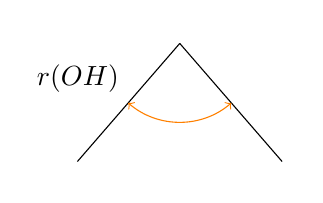
\begin{tikzpicture}
   \Odraw{0,1.5}
   \Hdraw{-1.3,0}
   \Hdraw{1.3,0}
%  \shade[inner color=blue,outer color=red] (0,0) rectangle (4,4);
%  \shadedraw[inner color=blue,outer color=red, draw=black] (0,0) rectangle (4,4);
  \draw(0,1.5) node[circle,minimum size=.4cm] (O) {};
  \draw(-1.3,0) node[circle,minimum size=.3cm,] (H1) {};
  \draw(1.3,0) node[circle,minimum size=.3cm,] (H2) {};
  %\draw(1.3,0) node[circle,minimum size=.2cm,draw,fill=blue] (H2) {};
  %\draw(.65,.8) node[circle,minimum size=.5cm,draw,fill=blue] (O) {};
 % \draw (A.center) -- (B.center);
\begin{pgfonlayer}{background}
 \draw (O.center) -- node[above left] {$r(\te{OH})$}(H1.center);
 \draw (O.center) --  (H2.center);
  \draw pic["$\anghoh$", draw=orange, <->, angle eccentricity=1.2, angle radius=1.cm]
    {angle=H1--O--H2};
\end{pgfonlayer}
 \end{tikzpicture}
\end{equation*}
 \caption{The geometry of $\tip$ water. O is red, H is blue. Each atom coincides with a site with charge $q$ and
  LJ-paramteres $\eps$ and $\si$.}
\label{Fig:Theo:TIP3Geo}
\end{figure} 

When there is no bond formation or breaking to be expected, quantum mechanical
calculations can be replaced by classical calculation, that is the position
of the atomic cores is again a sharply determinable quantity and motion
is governed by forces. That is, all particles move in a classical potential.
We will only treat water molecules as classical particles, so we need a good
%% CHECK: Real source by Jorgensen? Or 1981 source?
classical model of water. We decided on the quite popular $\tip$ potential 
by Jorgensen \etal \cite{Jorgensen1983TIP3P}. The geometry can be
seen in Figure \ref{Fig:Theo:TIP3Geo}. The three sites of the $\tip$ potential
coincide with the atoms forming $\hto$. Each site has a charge $\qal$ with 
\ep{Coulomb interaction}
\begin{equation}
\EC(\ralbe)=\frac{1}{4\pi\eps_0}\frac{\qal\qbe}{\ralbe},
\label{Theo:TIP3EC}
\end{equation}
where $\al,\be$ are the site types and $\ralbe$ is the distance between
the sites $\al$ and $\be$. Sites also interact by Van-der-Waals forces
which are described by a \ep{Lennard-Jones} (LJ) potential
\newcommand\ELJ{\enmat V^{\te{LJ}}_{\al\be}}
\newcommand\salbe{\enmat{\si_{\al\be}}}
\newcommand\ealbe{\enmat{\eps_{\al\be}}}
\begin{equation}
\ELJ(r)=4\ealbe\ed{\rb{\frac{\salbe}{\ralbe}}^{12}-\rb{\frac{\salbe}{\ralbe}}^{6}}.
\label{Theo:TIP3ELJ}
\end{equation}
The original $\tip$ model only had LJ interaction between the oxygen atoms. In
the CHARMM \cite{CHARMM} implementation, the H atoms are LJ sites as well. Therefore,
a $\tip$ water molecule $i$ moves in the potential of all other $\tip$ waters by
\begin{equation}
V_i(\r_i)=\sum_{j\neq i} \sum_{\al,\be} \ed{\EC(\ralbe(\r_i,\r_j)) + \ELJ(\ralbe(\r_i,\r_j))}.
\label{Theo:TIP3Potential}
\end{equation}
The first sum runs over all other water molecules and the second over all sites in both
molecules. \eqref{Theo:TIP3Potential} only contains intermolecular interaction. There
would also be the possibility to include intramolecular degrees of freedom with
harmonic potentials for bond and angle stretching. This is not the case for $\tip$,
where all sites are fixed within the molecule, reducing the 9-dimensional coordinate
\mbox{$\r_i=\r_i\rb{\r_{\te O},\r_{\te H1},\r_{\te H2}}$} to a 6-dimensional one, \mbox{$\r_i=\r_i\rb{\r_{\te O},\Om}$}
with the orientational dependency described by $\Om\in\R^3$.

The parameters $\ealbe$, $\salbe$ and $\qal, \qbe$ as well as the geometric parameters
$\r(\te{OH})$ and $\anghoh$ define the $\tip$ potential. They are chosen to reproduce
(macroscopic) thermodynamic properties of a pure water system.
%% CHECK if heats. Wikipedia nennt eine andere Quelle dafür.
The CHARMM $\tip$
potential is fitted to yield good specific heats \cite{MacKerell1998CHARMMTIP3}.  

\subsection{QM/MM}
\label{Sec:Theo:QMMM}

We already motivated using both QM and MM calculations simultaneously due to
the speed of MM and the accuracy of QM results. The simultaneous use
demands some notion of coupling between the two systems. The original
QM/MM coupling scheme proposed by Warshel and Levitt \cite{Warshel1976QMMM}
is nowadays only one among several schemes.
%% CHECK: Dringend checken, ob das irgendwie stimmt.
We chose an approximation
in which the QM part was subject to the external potential defined
by the MM charges and the MM part interacted with the QM atoms by
the LJ potential \eqref{Theo:TIP3ELJ}. That way, the electrostatic
interaction is covered by the QM part while the MM part accounts for
VdW interaction.

\subsection{Energy Minima and Transition States}
\label{Sec:Theo:Minima}
Finding energy minima of the PES for QM or QM/MM systems is basically following
the path defined by the gradient (force)
\newcommand\RM{\enmat{\bo R^M}}
\begin{equation}
\bo F(\RM)=-\nabla V(\RM)
\label{Theo:ForceGradient}
\end{equation}
of the total system's energy $V(\RM)$, where $\RM$ is the vector containing
all atomic coordinates. Again, there is no knowing whether this leads to
a global or a local minimum.

When working on a computer, \eqref{Theo:ForceGradient} must be integrated
in a discretised form. This is best done with step sizes depending on the
value of $\bo F$ and of course one needs tolerances that define convergence.
We used the $\dlfind$ algorithm \cite{Kaestner2009} with the default tolerances
to follow the minimum energy path.

Evaluating the gradient in \eqref{Theo:ForceGradient} is fortunately not
expensive in comparison to a single energy evaluation of the QM part. The gradient of
the MM region can be calculated straighforwardly from \eqref{Theo:TIP3Potential}.
For the QM region, there are schemes to obtain analytical results for the gradient
for a given wave function \cite{Brorsen2014AnalyticalGradientDFT}.
%% CHECK: do they ignore QM/MM?

%% CHECK: Pre-reactive complex?
\newcommand\ebased[2]{exp(-(\x-#1)^2/#2)} 
\begin{figure}[ht]
%\includegraphics{
\tikzsetexternalprefix{TikzPics/Theo/}
\tikzsetnextfilename{Fig.Theo.PES} 
\begin{equation*}
\begin{tikzpicture}
  \draw[->] (-3.7,0) -- (5,0) node[right] {$\xi$};
  \draw[->] (-3.4,-.3) -- (-3.4,4.5) node[above] {$E$};
  \draw[domain=-2.4:4.1,smooth,variable=\x,blue] plot ({\x}, {1+3*\ebased{1}{1.5}-1*\ebased{2}{.6}+2*\ebased{4}{3}});%{4*\ebased{2}{3}});
  \draw[domain=4.1:4.3,smooth,variable=\x,blue] plot ({\x}, {3.0});%{4*\ebased{2}{3}});
  \draw[dotted] (2.3,-.1) node[below] {$\xi_{\te {MIN}}$} -- (2.3,4.3) ;
  \draw (1.9,1.87) -- (2.7,1.87) node[right] {$E_{\te {MIN}}$};
  \draw[dotted] (.9,-.1) node[below] {$\xi_{\te {TS}}$} -- (.9,4.3) ;
  \draw (.5,3.93) -- (1.3,3.93) node[right] {$E_{\te {TS}}$};
  \draw[dotted] (-2.4,-.1) node[below] {$\xi_{0}$} -- (-2.4,4.3) ;
  \draw (-2.6,1.004) node[left] {$E_{0}$} -- (-2,1.004) ;
\end{tikzpicture} 
\end{equation*}
 \caption{A cut of a PES along reaction coordinate $\xi$. The reaction coordinate starts
 at some initial $\xi_0$ with energy $E_0$ and follows a path of minimum energy.
 The minimum with $E_{\te{MIN}}$ is located at $\xi_{\te{MIN}}$. The transition state with $E_{\te{TS}}$
 is a maximum at $\xi_{\te {TS}}$.}
\label{Fig:Theo:PES}
\end{figure} 

To evaluate our model, we will also calculate a \ep{transition state} (TS). This
is the state of maximum energy along a \ep{reaction path}, that is a path that
starts at some initial geometry with initial \ep{reaction coordinate} $\xi_0$
and then follows the negative gradient to a maximum (the transition state) and
after that reaches a new minimum by continuing on its route along the
gradient. In Figure \ref{Fig:Theo:PES}, an example of such a path between
reaction coordinates $\xi_0$ and $\xi_{\te{MIN}}$ is plotted. 

%% CHECK: ZITAT. Außerdem Theorie checken!
In this work, we obtain transition state with the \ep{dimer method} \cite{DimerMethod}. It uses two
images of the system with a slight offset, then rotates them to find the minimum 
eigenvalue of the Hessian matrix \eqref{Theo:Hessian}. It follows these ``gradients" 
by an iterative scheme a saddle point is reached. This is the transition state.

Transition states are important for calculating tunneling rates. These are interesting
for the analysis of molecule formation on ice surfaces since at temperatures as low
as in the interstellar medium, tunneling has a significant contribution to the dynamics of 
these systems.

\subsection{Technical Details}

%% CHECK: Sollte nwchem noch rein?
Before proceeding to actual calculations, we want to mention the programs and tools 
used for these. As we already mentioned, the optimisations are carried out with
$\dlfind$ \cite{Kaestner2009}, as are the dimer method and the calculation of 
Hessian matrices. DFT calculations are performed with TURBOMOLE\cite{TURBOMOLE}.
Force field calculations are performed by CHARMM \cite{CHARMM2009}. These programs were interfaced
via ChemShell \cite{chemshell}, which also provided the QM/MM coupling.

For the post-HF calculations in the benchmark, we used the MOLPRO \cite{MOLPRO_brief}
package.

All molecular visualisations are created with VMD \cite{HUMP96}.

%% CHECK: Mehr Details zum JUSTUS?
The calculations were performed on the bwForCluster JUSTUS of the German federal country
of Baden-Württemberg. Shared memory parallel calculations with up to 16 CPUs
were performed. The main limit was the maximal computation time of six days.


%\subsection{The Fletcher Surface}
%\label{Sec:Theo:Fletcher}

\section{Benchmarking}
\newcommand\htohto{\mbox{\enmat{\hto-\hto}}}
\newcommand\htoo{\mbox{\enmat{\hto-\hspace{.2pt} ^3\te{O}}}}
\newcommand\htoh{\mbox{\enmat{\hto-\te H}}}
\label{Sec:Bench}

In the previous section, we did introduce the basic notions of the theoretical structure underlying our
computations. We did already mention that the choice of DFT functionals and basis sets is of great importance
to the accuracy of our calculations. Unfortunately, not much can be said a priori about
which functional combined with which basis set should be used to describe a certain system.
There are recommendations as some functionals were fitted to best represent a certain
group of elements or reactions, but in order to determine the reliability of the
later results, there is no way around literature research and own benchmark tests.

We already
discussed the functionals we want to test in Section \ref{Sec:Theo:Functionals}, and we
have reason to hope that at least the \pbez, $\pw\dt$ and $\bns\dt$ functionals will be sufficiently
accurate to describe water-water interaction, as they are recommended by Anacker and Friedrichs \cite{Anacker2014}.
We did also already name the basis sets we want to compare alongside the functionals in Section \ref{Sec:Theo:Basis}.

We used three different benchmarks, namely the interaction energies of an $\htoh$, an $\htohto$ and an $\htoo$ system.
The reference calculations were in all cases performed with the MOLPRO \cite{MOLPRO_brief} package
at the $\ccsdtf$ \cite{CCSDTF12} level of theory with the $\vtz$\cite{VTZ} basis set, for
which we found energy minima \footnote{In the $\htoo$ case, a first minimum was calculated at the
$\mrcif/\vtz$ \cite{MRCIF12} level of theory, where it was found that the wavefunction can be well
described by a single-reference method. From there, the $\ccsdtf$ minimisation was carried out.}.
For $\htoo$, the $\ccsdtf$ calculations were preceded by \ep{multi-reference}\cite{Multiref} calculation
at the $\mrcif/\vtz$ level of theory to find an optimum geometry, which turned out to be
suitable for single-reference treatment.

At each optimum geometry, an additional calculation was carried out to find a CP
corrected energy. For $\htoh$ and $\htohto$, this calculations was also at the $\ccsdtf/\vtz$ level
of theory, while for the $\htoo$ interaction again an $\mrcif/\vtz$ calculation with
Davidson correction\cite{DavidsonCorrection} was
required due to the necessity of a multireference treatment of the case where the
$^3\te O$ radical is set as a dummy atom. In all cases, the $\vtz$ basis set is 
large enough to require only small CP corrections of $0.05 - 0.18 \ \kmo$. 
%We used these minima as initial geometries for two different
%types of reference calculations:
%% CHECK: Sollte man Benchmark i. überhaupt erwähnen? Meine Schlussfolgerung: Nein.
%\begin{enumerate}[i.]
%  \item Energy reference: No minimisation was performed. Instead, the $\ccsdtf/\vtz$ geometries
%    were used and the energy values are compared.
%  \item Geometry reference: The initial geometries were further optimized to arrive at a minimum
%    geometry and energy corresponding to the DFT method.
%\end{enumerate}

We performed energy minimisations at the DFT level of theory with different basis sets. The initial
geometry was always the reference geometry provided by the $\ccsdtf$ calculation. The results can be compared
to the coupled-cluster data with respect to optimum geometry and energy deviations. We will discuss
these for the three test systems separately.

The deviation of optimum geometry \mbox{$\bo R^M\dft=(\r^1\dft,\ldots,\r^M\dft)$} from the reference optimum geometry 
\mbox{$\bo R^M\cc=(\r^1\cc,\ldots,\r^M\cc)$} can be quantified by the \ep{root mean square deviation} (RMSD). It
is given by
\newcommand{\DRMSD}{\Dl_{\te{RMSD}}}
\begin{equation}
\Dl_{\te{RMSD}}(\bo R^M\dft;\bo R^M\cc)=\sqrt{\frac 1 M \sum_{k=1}^M \abs{\r^k\dft-\r^k\cc}^2}.
\label{Bench:RMSD}
\end{equation}
We will give $\DRMSD$ in $\Ang$.   

%% CHECK: Source?
Note that, obviously, the coupled cluster results are approximations just as the DFT results, however
there is good reason to assume that they are more accurate. For the following comparisons, we will
therefore consider the coupled cluster results as if they were the correct values for this
interaction.

%% CHECK: Speedup-table?
Another remark before starting the benchmark is the accuracy with which numerical
integration was carried out. In the TURBOMOLE code, we used an m4 integration grid
with keyword ``\$scfconv 8''. The results were compared to the more accurate
m5 grid and ``\$scfconv 9'', which meant no change in energy. Therefore, we recommend
the slightly less accurate integration technique due to it being computationally
faster. 

\subsection{$\htoh$ Interaction}

\tikzsetexternalprefix{TikzPics/Benchmark/}
\tikzsetnextfilename{Fig.Bench.H2O+H.NoD3}
\pgfplotsset{xtick style={draw=none}}
\begin{figure}[h]
\centering
\begin{tikzpicture}
\begin{axis}[
    height=8cm,
    width=.48*\textwidth,
    ybar,
    xmin=.5,
    xmax=9.5,
    ymin=-.7,
    ybar=0pt,
    axis x line*=bottom,
    enlarge x limits=0.015,
    enlarge y limits=0.15,
    legend style={legend pos=south west,font=\small,legend columns=1},
    ylabel={interaction energy deviation $\Delta \eint$ / kJ/mol},
    xticklabels={\btlyp,\bns,\bhlyp,\blyp,\bp,\pbe,\pbez,\tpssh,\pw},
    xtick=data,
    grid=minor,
    xticklabel style={rotate=90},
    bar width = .008*\textwidth,
    minor xtick={1.5,...,8.5},
    yticklabel pos=left,
    grid style={dotted,gray},
    ymajorgrids=true,
    ]
\addplot[green!20!black,fill=green!80!white] coordinates {(1,-.17957936646) (2,.36521188354) (3,-.07314159646) (4,-.13145395146) (5,-.02562004646) (6,-.61493977646) (7,-.15329811146) (8,.02935792354) (9,-.32041118646) };
\addplot[blue!20!black,fill=blue!80!white] coordinates {(1,-.09364675146) (2,.38435177854) (3,-.01343772646) (4,-.05111365146) (5,.03597418354) (6,-.44399347146) (7,-.07471689646) (8,.01756942854) (9,-.20565058146) };
\addplot[red!20!black,fill=red!80!white] coordinates {(1,.19741617854) (2,.35121796854) (3,.18210951354) (4,.39813565354) (5,.23267664354) (6,-.19932312646) (7,.09974757854) (8,.23782262354) (9,.03978115854) };
\addplot[yellow!20!black,fill=yellow!80!white] coordinates {(1,.06989564354) (2,.35788673854) (3,.11838862854) (4,.18512883854) (5,.12862807854) (6,-.28819630146) (7,.04897040854) (8,.12219560354) (9,-.03386411646) };

%\addplot[green!20!black,fill=green!80!white] coordinates {(1,-1.38867462646) (2,.35885817354) (3,-.79392011146) (4,-1.88993508646) (5,-2.70903857646) (6,-1.89731274146) (7,-.85296760646) (8,-7.27761861646) (9,-5.38880766146) (10,-.34732256146) };
%\addplot[blue!20!black,fill=blue!80!white] coordinates {(1,-.45181746146) (2,.40364920354) (3,-.14531659146) (4,-.86748662146) (5,-3.06760311146) (6,-.56095949646) (7,-.09096874146) (8,-8.76869257646) (9,-6.56655445146) (10,-.21066528646) };
%\addplot[red!20!black,fill=red!80!white] coordinates {(1,.13821115354) (2,.35153302854) (3,.15884758354) (4,.31267562854) (5,-2.18406985146) (6,-.85294135146) (7,-.24025467146) (8,-7.37633741646) (9,-5.39749806646) (10,-.02593510646) };
%\addplot[yellow!20!black,fill=yellow!80!white] coordinates {(1,-.18921495146) (2,.38823751854) (3,.03639426354) (4,-.31846831646) (5,-2.69564852646) (6,-.73300851146) (7,.01846209854) (8,-8.12079794146) (9,-6.01869136646) (10,-.09808384646) };
\legend{def2-SVPD,def2-TZVP,def2-TZVPD,def2-QZVP}
\end{axis}
\end{tikzpicture}
%\captionsetup{format=hang}
%\setcapmargin[4cm]{1cm}
\caption{The $\htoh$ benchmark results for different basis sets without dispersion correction.
Energies are plotted as differences to the reference energy from $\ccsdtf/\vtz$ calculations,
see \eqref{Bench:RefEnergy}.}
\label{Fig:Bench:H2O+H:NoD3}
\end{figure}

First information about $\htoh$ interaction can be found in Figure \ref{Fig:Bench:H2O+H:NoD3}
and Figure \ref{Fig:Bench:H2O+H:D3}, where
we compared functionals (with and without dispersion correction, respectively) in different basis sets. We compared
energy values of the form
\newcommand\ecc{\enmat{\eint_{\te {CC}}}}
\begin{equation}
\Dl\eint=\eint\dft-\ecc.
\label{Bench:RefEnergy}
\end{equation}
$\eint\dft$ stands for the interaction energy \eqref{Theo:InteractionEnergy} of the system computed with a certain
DFT functional and basis set, and $\ecc$ is the CP corrected interaction energy with $\ccsdtf/\vtz$.
For $\htoh$, we found \mbox{$\ecc=-0.40\ \kmo$}, so we have an only
weakly bonded system. The CP correction contributes $+0.05\ \kmo$ to
the energy.

Before discussing different functionals and the dispersion corrections, we can have a look
at the differences between the four basis sets used.Figure \ref{Fig:Bench:H2O+H:NoD3} does not contain our results
for the def2-SVP basis set since they are much worse than all other results --
up to $-20\ \kmo$ and usually more than $-5\ \kmo$ of deviation. Only the $\bhlyp$, $\pbez$ and
$\pw$ functional had errors between $-2$ and $-5$ $\kmo$ with def2-SVP. However,
the addition of diffuse functions effects quite a remarkable improvement to the
def2-SVP results, such that def2-SVPD calculations are well comparable to 
results obtained by basis sets of more than double-$\zeta$ order.

It is also
noteworthy that def2-QZVP does not seem to offer a clear advantage over the
other three basis sets in both figures. With additional dispersion,
it tends to yield similar accuracy as def2-TZVP, while usually being inferior
to def2-TZVPD for most functionals. Still, without dispersion correction,
its accuracy is between def2-TZVP and def2-TZVPD and only rarely better
than both. def2-QZVP takes approximately 1.5 times as long to complete a single
SCF iteration as def2-TZVPD. From a first glance
at the ``better'' functionals in this case, one could therefore consider
the def2-TZVP and def2-TZVPD basis sets as good compromises between
accuracy and computational cost. 

\tikzsetexternalprefix{TikzPics/Benchmark/}
\tikzsetnextfilename{Fig.Bench.H2O+H.D3}
\begin{figure}[h]
\centering
\begin{tikzpicture}
\begin{axis}[
    height=8cm,
    width=.48*\textwidth,
    ybar,
    xmin=.5,
    xmax=9.5,
    ybar=0pt,
    axis x line*=bottom,
    enlarge x limits=0.015,
    enlarge y limits=0.15,
    legend style={legend pos=south west,font=\small,legend columns=1},
    ylabel={interaction energy deviation $\Delta \eint$ / kJ/mol},
    xticklabels={\btlyp\dt,\bns\dt,\bhlyp\dt,\blyp\dt,\bp\dt,\pbe\dt,\pbez\dt,\tpssh\dt,\pw\dt},
    xtick=data,
    grid=minor,
    xticklabel style={rotate=90},
    bar width = .008*\textwidth,
    minor xtick={1.5,...,8.5},
    yticklabel pos=left,
    grid style={dotted,gray},
    ymajorgrids=true,
    ]
 \addplot[green!20!black,fill=green!80!white] coordinates {(1,-2.39332220146) (2,.33675146354) (3,-.76816395646) (4,-2.85861331146) (5,-5.18753683146) (6,-1.37496951646) (7,-.86554375146) (8,-.85577689146) (9,-.66041343646) };
\addplot[blue!20!black,fill=blue!80!white] coordinates {(1,-2.17766363146) (2,.32630197354) (3,-1.22998940646) (4,-4.40490153646) (5,-6.08159834646) (6,-1.20436452646) (7,-.78775018646) (8,-.86803797646) (9,-.54581036146) };
\addplot[red!20!black,fill=red!80!white] coordinates {(1,-2.12935443146) (2,.32170734854) (3,-.51228272646) (4,-3.21961956146) (5,-5.29358077646) (6,-.95937912146) (7,-.61265559146) (8,-.64757474146) (9,-.29990603146) };
\addplot[yellow!20!black,fill=yellow!80!white] coordinates {(1,-1.96625837146) (2,.35990837354) (3,-.57660747646) (4,-3.79917243146) (5,-5.74679458646) (6,-1.04856735646) (7,-.66372156646) (8,-.76354307646) (9,-.37368258146) };

%\addplot[green!20!black,fill=green!80!white] coordinates {(1,-1.97799435646) (2,.32338766854) (3,-1.22313685146) (4,-3.62034962646) (5,-3.92406746646) (6,-2.72187727146) (7,-1.68002636146) (8,-9.09123525146) (9,-7.27662092646) (10,-.69927083646) };
%\addplot[blue!20!black,fill=blue!80!white] coordinates {(1,-2.78000584146) (2,.32165483854) (3,-1.43427956146) (4,-4.40482277146) (5,-6.08157209146) (6,-1.46258245146) (7,-.92795188646) (8,-10.45730915646) (9,-8.34535695646) (10,-.56957113646) };
%\addplot[red!20!black,fill=red!80!white] coordinates {(1,-1.53727792646) (2,.32107722854) (3,-1.13329224146) (4,-3.21954079646) (5,-5.29355452146) (6,-1.65534666146) (7,-1.02512164146) (8,-9.05471454646) (9,-7.20799035646) (10,-.30591842646) };
%\addplot[yellow!20!black,fill=yellow!80!white] coordinates {(1,-2.45502145146) (2,.35329211354) (3,-1.26023516646) (4,-3.79922494146) (5,-5.74687335146) (6,-1.38919972646) (7,-1.00191222146) (8,-9.77473166646) (9,-7.77722501146) (10,-.39245490646) };
\legend{def2-SVPD,def2-TZVP,def2-TZVPD,def2-QZVP}
\end{axis}
\end{tikzpicture}
\caption{The $\htoh$ benchmark results for different basis sets including dispersion correction.
Energies are plotted as differences to the reference energy from $\ccsdtf/\vtz$ calculations,
see \eqref{Bench:RefEnergy}.}
\label{Fig:Bench:H2O+H:D3}
\end{figure}

The first general result on functionals is that the inclusion
of the D3 dispersion correction is not beneficial to the interaction
energy values of $\htoh$, which can be seen by comparing Figure \ref{Fig:Bench:H2O+H:NoD3}
to Figure \ref{Fig:Bench:H2O+H:D3}. Indeed, while most functionals without
dispersion corrections have errors of between $-0.2$ and $0.2\ \kmo$ for at
least one basis set, the D3 corrected versions deviate stronger than $-5\ \kmo$.
The contribution of dispersion in $\htoh$ is therefore strongly overestimated by the
D3 correction. The best results for dispersion corrected functionals are obtained
by $\pw\dt/\tzvpd$ with a deviation of $-0.30\ \kmo$.

We will therefore mainly focus on the data in Figure \ref{Fig:Bench:H2O+H:NoD3}. 
The results here tend to be very accurate.
%% CHECK: Accuracy ccsd(t)?
In fact, the deviations are within the error bonds of a $\ccsdtf$ calculation,
so it is hard to favor a functional of the given choice. Still, at least two
functionals need special remarks, but rather for their deficiencies. The first one
are the $\tpss$ and $\tpss\dt$ functionals. They predict much too attractive energies
for this benchmark, beyond $-7\ \kmo$ and $-9\ \kmo$, respectively. 
%% CHECK: Vergleich, ob das jedesmal etwa derselbe Abstand ist (basis- und dispersionsabhängig).
They predict
a wrong optimum geometry, where the H radical is at a distance of around $2.20\ \Ang$
from the O atom in the water molecule, which is much less than the reference
value of $3.34\ \Ang$.

The opposite problem happens for $\bns$ and $\bns\dt$ optimisations. Here, the attraction is
considered close to being repulsive, with interaction energy values around
\mbox{$\eint_{\bns}\approx -0.03\ \kmo$}. While the resulting deviation of around
$0.37\ \kmo$ does not look too dramatic in Figures \ref{Fig:Bench:H2O+H:NoD3} and
\ref{Fig:Bench:H2O+H:D3}, it is a qualitative mistake. The separation between
radical H and water O is around $5.80\ \Ang$, which is close to describing two isolated
systems.

Comparing RMSD data of different functionals yields similar results as the energy comparison.
Functionals without the D3 correction
predict very accurate geometries with $\DRMSD < 0.01\ \Ang$ for all but $\tpss$ and $\bns$.
Despite worse energy results, many D3 corrected versions still find accurate optimum geometries.
Exclusions are $\btlyp\dt$, $\blyp\dt$, $\bp\dt$, which do find optima similar to the already mentioned
$\tpss$ optimum, with the H radical too close to the water O. The $\bhlyp$ functional
generally yields good geometries, only for the $\tzvp$ basis set it also predicts the H
radical too close to the water O.

Concerning the change of optimum geometry with respect to the choice of basis set, most
basis sets lead to the same optimum geometry for nearly all functionals. Only the
$\svp$ basis set and the $\tzvpp$ basis set often lead to wrong, i.e. too
attractive, geometries. 

% Let us now look at the different functionals. The $\bns$ functional
% seems to offer a very good approximation to $\ecc$  with and without dispersion
% correction. This is unfortunately not due to the functional's accuracy but instead
% it appears that the functional
% considers the $\htoh$ interaction to be repulsive in the region where most functionals
% find an energy minimum, so it finds a less attractive optimum geometry at
% a much larger distance between the water oxygen and the hydrogen atom.
% A more satisfactory result is produced with the $\pw$ functional. The energies 
% are very accurate both for $\pw$ and $\pw\dt$ and they do not vary strongly with basis set size.
% They are most accurate for the def2-TZVPD basis set with a deviation
% of only $\Dl\eint=-0.025 \kmo$ (no D3 correction) and $\Dl\eint=-0.255 \kmo$ (D3 corrected).
% %The def2-TZVPD basis set is computationally much
% %faster than the def2-QZVP basis set (which takes roughly 1.5 times
% %the computation time of the smaller basis set). 
% For basis sets
% larger than def2-SVPD the $\btlyp$, $\bhlyp$ and $\pbez$ functionals yield very good
% results as well, although the dispersion corrected version are significantly less accurate.
% The $\tpss$ and $\tpssh$ functionals should not be used to describe this interaction,
% while $\btlyp$ and $\blyp$ can be considered quite good -- not as good as
% $\pw$, $\bhlyp$ or $\pbez$ but much better than $\tpss$ and $\tpssh$ -- while they become
% worse with additional dispersion.
% 
% So from the $\htoh$ data, one can already conclude that the $\tpss$ and $\tpssh$
% functionals should not be expected to yield good energy values for hydrogen adsorption,
% which may however still occur due to error cancellation. The $\bns$ functional
% is probably also not fit to describe such a system accurately. Furthermore, the def2-SVP basis
% set is not fit to describe $\htoh$ interaction. Since they are sufficiently accurate
% while not too expensive, we will especially evaluate the def2-TZVP basis set family
% for $\htohto$ interaction.
%% CHECK: Table mit Computation times?
%% CHECK: RMSD table?

\tikzsetexternalprefix{TikzPics/Benchmark/}
\tikzsetnextfilename{Fig.Bench.H2O+H2O.TZVPCompare}
\begin{figure}[h]
\centering
\begin{tikzpicture}
\begin{axis}[
    height=8cm,
    width=.48*\textwidth,
    ybar,
    xmin=.5,
    xmax=10.5,
    ybar=0pt,
    axis x line*=bottom,
    enlarge x limits=0.015,
    enlarge y limits=0.15,
    legend style={legend pos=north east,font=\small,legend columns=2},
    ylabel={interaction energy deviation $\Delta \eint$ / kJ/mol},
    xticklabels={\btlyp,\bns,\bhlyp,\blyp,\bp,\pbe,\pbez,\tpss,\tpssh,\pw},
    xtick=data,
    grid=minor,
    xticklabel style={rotate=90},
    bar width = .008*\textwidth,
    minor xtick={1.5,...,9.5},
    yticklabel pos=left,
    grid style={dotted,gray},
    ymajorgrids=true,
    ]
\addplot[blue!20!black,fill=blue!80!white] coordinates {(1,-2.4712713930) (2,1.8105515370) (3,-3.4503203430) (4,-1.5251462130) (5,-1.4308382530) (6,-5.0817010230) (7,-3.9391359330) (8,-2.3940816930) (9,-2.2228465830) (10,-2.6678163230) };
\addplot[red!20!black,fill=red!80!white] coordinates {(1,1.4702867370) (2,5.7188708370) (3,-.1324234830) (4,3.0175463970) (5,2.6200456970) (6,-.7830223830) (7,-.2683193630) (8,1.5256322770) (9,1.5457961170) (10,1.0097740370) };
\addplot[blue!20!black,pattern color=blue!80!white,pattern = horizontal lines] coordinates {(1,-5.5127031030) (2,-3.4044266030) (3,-5.8857341430) (4,-5.2560342230) (5,-4.9150342830) (6,-6.9246970030) (7,-5.8901449830) (8,-4.9479580530) (9,-4.7306191630) (10,-4.0300832530) };
\addplot[red!20!black,pattern color=red!80!white,pattern = horizontal lines] coordinates {(1,-1.5693596330) (2,.6348001270) (3,-2.5674172030) (4,-.7562947930) (5,-.8699789430) (6,-2.5687824630) (7,-2.2220064230) (8,-.9511594030) (9,-.9633417230) (10,-.3517577530) };
%\addplot[blue!20!black,fill=blue!80!white] coordinates {(1,-2.2911688300) (2,1.8945608000) (3,-3.3056620300) (4,-1.3177384500) (5,-1.2830293400) (6,-4.9496451100) (7,-3.7824003200) (8,-2.2352456800) (9,-2.0561340700) (10,-2.4866635600) };
%\addplot[red!20!black,fill=red!80!white] coordinates {(1,1.6138948500) (2,5.9163017000) (3,.0413778800) (4,3.1551158600) (5,2.9033304100) (6,-.6073831700) (7,-.1202479000) (8,1.6705531400) (9,1.6996436800) (10,1.2347726500) };
%\addplot[blue!20!black,pattern color=blue!80!white,pattern = horizontal lines] coordinates {(1,-5.3662069400) (2,-3.1298060400) (3,-5.7434387800) (4,-5.0291977600) (5,-4.7869166200) (6,-6.8055060400) (7,-5.7431237200) (8,-4.8009367900) (9,-4.5759839500) (10,-3.8439420400) };
%\addplot[red!20!black,pattern color=red!80!white,pattern = horizontal lines] coordinates {(1,-1.4527941700) (2,.9033820400) (3,-2.3888899400) (4,-.5200065300) (5,-.7710043300) (6,-2.4600935000) (7,-2.0844369600) (8,-.8217289900) (9,-.8236718600) (10,-.1117937900) };
\legend{def2-TZVP,def2-TZVPD,def2-TZVP+D3,def2-TZVPD+D3}
\end{axis}
\end{tikzpicture}
\caption{The $\htohto$ benchmark results for the def2-TZVP and def2-TZVPD basis sets.
The results with dashed bars include dispersion corrections. Energies are plotted as differences
to the reference energy from $\ccsdtf/\vtz$ calculations, see \eqref{Bench:RefEnergy}.}
\label{Fig:Bench:H2O+H2O:TZVPCompare}
\end{figure}

\subsection{$\htohto$ Interaction}

Again, we compare energies to the reference energy as in \eqref{Bench:RefEnergy}. The
reference energy for the $\htohto$ dimer is at \mbox{$\ecc=-20.80\ \kmo$}, where
the CP correction contributes $+0.18\ \kmo$.
In Figure \ref{Fig:Bench:H2O+H2O:TZVPCompare}, we take a look at the differences between
dispersion corrected and not dispersion corrected results in the def2-TZVP and def2-TZVPD
basis sets. The stronger attraction between the two $\hto$ molecules does prevent
errors as for the $\bns$ functional in the previous section, so all functionals
expect attractive interaction. Inclusion of the D3 dispersion correction does again
predict stronger attraction, while the additional diffuse functions of the
def2-TZVPD basis set weaken the attraction. These effects can combine to
yield good results, for example for $\bns\dt$ or $\pw\dt$.
%the high accuracy of $\pw\dt$ with the def2-TZVPD basis set. 

%Dispersion corrections , this may well be due to the more important role of dispersion for this interaction. 
The inaccuracy of some functionals may be due to the bad treatment of
dispersion in DFT. But inclusion of the D3 correction does not resolve the issue for cases
where the interaction is already too attractive. This
is most striking for the def2-TZVP basis set, which predicts too attractive
interaction for all functionals but $\bns$. Generally, every functional has its
most accurate results -- either in the standard or the dispersion corrected version --
at the def2-TZVPD basis set. This was also very accurate for $\htoh$ interaction,
so this benchmark confirms it as a good choice of basis set. Excellent
results at the $\tzvpd$ level are obtained by $\bhlyp$, $\pbez$ and $\pw\dt$,
but they are all not too accurate in the $\tzvp$ basis set.  


% Another
% result that reappears is the good accuracy of the $\bhlyp$ and $\pbez$ functional
% without dispersion correction in the def2-TZVPD basis set, however both are
% not too accurate with def2-TZVP. Another very good functional is 
% the already mentioned $\pw\dt$, which is also only strikingly good with
% def2-TZVPD. 

\tikzsetexternalprefix{TikzPics/Benchmark/}
\tikzsetnextfilename{Fig.Bench.H2O+H2O.BasisCompare}
\begin{figure}[h]
\centering
\begin{tikzpicture}
\begin{axis}[
    height=8cm,
    width=.493*\textwidth,
    ybar,
    xmin=.5,
    xmax=3.5,
    ybar=0pt,
    ymax=2.5,
    axis x line*=bottom,
    enlarge x limits=0.015,
    enlarge y limits=0.15,
    %legend pos=south east,
    legend style={legend pos=north west,font=\small,legend columns=3},
    ylabel={interaction energy deviation $\Delta \eint$ / kJ/mol},
    xticklabels={\bhlyp,\pbez,\pw\dt},
    xtick=data,
    grid=minor,
    %xticklabel style={rotate=90},
    bar width = .010*\textwidth,
    minor xtick={1.5,2.5},
    minor ytick={-4,...,2},
    yticklabel pos=left,
    grid style={dotted,gray},
    ymajorgrids=true,
    ]


\addplot[green!20!black,fill=green!80!white] coordinates {(1,-1.9936404330) (2,-2.2264697730) (3,-2.3673015930) };
\addplot[blue!20!black,fill=blue!80!white] coordinates {(1,-3.4503203430) (2,-3.9391359330) (3,-4.0300832530) };
\addplot[brown!20!black,fill=brown!80!white] coordinates {(1,-1.9095719230) (2,-2.4086269630) (3,-2.5282447430) };
\addplot[red!20!black,fill=red!80!white] coordinates {(1,-.1324234830) (2,-.2683193630) (3,-.3517577530) };
\addplot[orange!20!black,fill=orange!80!white] coordinates {(1,.2438106670) (2,.1062344670) (3,.0347158470) };
\addplot[yellow!20!black,fill=yellow!80!white] coordinates {(1,-.5243581230) (2,-.9162402530) (3,-.9979458130) };
\addplot[purple!20!black,fill=purple!80!white] coordinates {(1,.2676502070) (2,.1384230970) (3,.0622835970) };
\legend{def2-SVPD,def2-TZVP,def2-TZVPD,def2-TZVPP,def2-TZVPPD,def2-QZVP,def2-QZVPD}

\end{axis}
\end{tikzpicture}
\caption{The $\htohto$ benchmark results for $\bhlyp$, $\pbez$ and $\pw\dt$ and all
basis sets used in the study (excluding \mbox{def2-SVP}). Energies are plotted as differences
to the reference energy from $\ccsdtf/\vtz$ calculations, see \eqref{Bench:RefEnergy}.}
\label{Fig:Bench:H2O+H2O:BasisCompare}
\end{figure}

We use these three most promising functionals to investigate the difference
between basis sets in Figure \ref{Fig:Bench:H2O+H2O:BasisCompare}. Only the def2-SVP basis set is not
considered, since it yields errors of between $-12\ \kmo$ and $-15\ \kmo$ for all three
functionals. The figure shows that while increasing the $\zeta$-order of the basis set
does indeed improve the results, inclusion of additional diffuse functions seems to
be even more beneficial. The basis set def2-SVPD is more accurate than def2-TZVP and
def2-TZVPD is more accurate than def2-QZVP.
%% CHECK! Does that make sense? Citation?
This may well be due to reduction of the BSSE, which depends on the ability
of basis sets to describe electrons far from the core.
The inclusion of polarisation functions as in def2-TZVPP does
also affect the results positively, however not to the extent of additional
diffuse functions. The def2-TZVPPD basis set is again an improvement
to the def2-TZVPP basis set, it is also stronger than the def2-TZVPD
basis set. Indeed, for all three functionals the def2-TZVPPD and
def2-QZVPD results are strikingly close to one another, which could
be an indication that the basis set truncation error is low and that
the intrinsic quality of the methods is reached. In that case, the
three methods of Figure \ref{Fig:Bench:H2O+H2O:BasisCompare} are all
capable of yielding excellent approximations to our coupled-cluster data,
and the results at the def2-TZVPD basis set are already close to the
methods' intrinstic error.  

%% CHECK: Sollte das hier kommen? Sollen wir nicht später darauf zurückkommen oder es früher
% erwähnen?
The results so far speak in favor of the def2-TZVPD basis set. Due 
to the size of the quantum mechanical part of the QM/MM system we will later consider,
it is computationally too expensive to use for the whole
QM part. We will therefore use a hybrid system with the more important atoms described by the def2-TZVPD
basis set and the less important ones by the def2-TZVP basis set. We will describe this
further subdivision of the QM domain in more detail in Section \ref{Sec:Ads:Model}.
We should therefore determine functionals that are both good for def2-TZVP and def2-TZVPD,
while their accuracy for def2-TZVPD is more important since the adsorption site will
be closer to the def2-TZVPD atoms. Figure \ref{Fig:Bench:H2O+H2O:TZVPCompare} shows
that good compromises between the two basis sets
are given by $\btlyp$, $\tpss$, $\tpssh$ and $\pw$, which all give mediocre results in
both basis sets. $\bhlyp$, $\pbez$ and $\pw\dt$ are highly accurate for def2-TZVPD but not very good
with def2-TZVP. $\bns\dt$ is somewhat between those functionals, being less accurate for 
def2-TZVPD but still better for def2-TZVP. All other functionals are
not accurate enough for def2-TZVP or def2-TZVPD.

For $\htohto$, the RMSD values are entirely unproblematic for any basis set beyond
$\svp$. The worst RMSD is reached by $\bns\dt/\tzvpd$, it is of \mbox{$0.076\ \Ang$},
which is just a slight displacement of H atoms. Especially $\btlyp$ and $\pw$ both
with and without dispersion corrections predict RMSDs of less than $0.008\ \Ang$
to the reference geometry, $\bhlyp$ is rougly at $0.010\ \Ang$ and the
rest is between $0.02$ and $0.05\ \Ang$. Therefore, $\htohto$ interaction geometries
are well described by any functional in a basis set bigger than $\svp$.

% With these hybrid basis set considerations, we can therefore nominate seven functionals
% that may describe water-water interaction in our context sufficiently accurate. If we exclude
% those that have proven very inaccurate for $\htoh$ interaction in these basis sets, we are
% left with only five, $\btlyp$, $\bhlyp$, $\pbez$, $\tpssh$ and $\pw\dt$. We might be able
% to narrow this selection down by considering the third benchmark. 

\subsection{$\htoo$ Interaction}

It already became clear at the beginning of this section that $\htoo$ interaction is
more tricky for post-HF methods because some geometries in the optimisation process
are not well described by a single Slater determinant. At the optimum geometry,
a single-reference approach is fortunately possible, so our results for this
benchmark have the full credibility of the $\ccsdtf$ method. Only the CP
correction is taken from an $\mrcif$ calculation, but it is as small as
\mbox{$0.10\ \kmo$} and therefore unlikely to deteriorate our results.
The CP corrected interaction energy is \mbox{$\ecc=-6.72\ \kmo$}.

% \pgfplotsset{
% % override style for non-boxed plots
%     % which is the case for both sub-plots
%     every non boxed x axis/.style={} 
% }
% \tikzsetexternalprefix{TikzPics/Benchmark/}
% \tikzsetnextfilename{Fig.Bench.H2O+O.TZVPCompare}
% \begin{figure}[h]
% \centering
%  \begin{tikzpicture}
% \begin{groupplot}[
%     group style={
%         group name=my fancy plots,
%         group size=1 by 2,
%         xticklabels at=edge bottom,
%         vertical sep=0pt
%     },
%     height=8cm,
%     width=.48*\textwidth,
% %     ybar,
% %     xmin=.5,
% %     xmax=10.5,
% %     %ymax=9.5,
% %     ybar=0pt,
% %     axis x line*=bottom,
% %     enlarge x limits=0.015,
% %     enlarge y limits=0.15,
% %     legend pos=north west,
% %     legend style={legend columns=2},
% %     ylabel={interaction energy deviation $\Delta \eint$ / kJ/mol},
% %     xticklabels={\btlyp,\bns,\bhlyp,\blyp,\bp,\pbe,\pbez,\tpss,\tpssh,\pw},
% %     xtick=data,
% %     grid=minor,
% %     xticklabel style={rotate=90},
% %     bar width = .008*\textwidth,
% %     minor xtick={1.5,...,9.5},
% %     yticklabel pos=left,
% %     grid style={dotted,gray},
% %     ymajorgrids=true,
%     ]
% \nextgroupplot[ymax=-12,
%                %ytick={60,80},
%                % 
%                axis y discontinuity=parallel,
%                height=3.5cm]
% \nextgroupplot[ymin=-5,ymax=9.5,
% axis x line=bottom,
% ]
% \addplot[blue!20!black,fill=blue!80!white] coordinates {(1,-.1081968550) (2,-9.0107947650) (3,-.2511553300) (4,-17.9176722400) (5,-15.0656966100) (6,-20.1429410200) (7,-.9848250500) (8,-.8730050050) (9,-.0743016500) (10,-.5862478950) };
% \addplot[red!20!black,fill=red!80!white] coordinates {(1,.4817004850) (2,1.1639366600) (3,.0664251500) (4,-4.9605409350) (5,-2.9669987850) (6,-16.2942468250) (7,-.5893722400) (8,-.1660366200) (9,.5068527750) (10,-.0768746400) };
% \addplot[blue!20!black,pattern color=blue!80!white,pattern = horizontal lines] coordinates {(1,-2.0464984850) (2,-15.1573265600) (3,-1.8328878050) (4,-21.1657045450) (5,-17.8578633500) (6,-21.2442857600) (7,-2.1535663750) (8,-2.4432115350) (9,-1.6152863650) (10,-1.5014446850) };
% \addplot[red!20!black,pattern color=red!80!white,pattern = horizontal lines] coordinates {(1,-1.4555772000) (2,-2.2273166700) (3,-1.5145721850) (4,-17.4665588300) (5,-15.0122414300) (6,-17.6048439150) (7,-1.6649345700) (8,-1.6973069850) (9,-1.0344207450) (10,-.9915725850) };
% % \addplot[blue!20!black,fill=blue!80!white] coordinates {(1,-3.2642316400) (2,-8.9154103500) (3,-.1969912650) (4,-17.8199248750) (5,-14.9692619950) (6,-20.0472940550) (7,-.1117675350) (8,-9.5628061400) (9,-2.8443879350) (10,3.2840804200) };
% % \addplot[red!20!black,fill=red!80!white] coordinates {(1,-1.2195447500) (2,-5.8266408750) (3,.0822569150) (4,-13.8070844200) (5,-11.7862370700) (6,-16.1985998600) (7,-.5081655250) (8,-6.8218629050) (9,-.8746065600) (10,-.3388207750) };
% % \addplot[blue!20!black,pattern color=blue!80!white,pattern = horizontal lines] coordinates {(1,-6.3561779700) (2,-15.0561660450) (3,-1.7440671400) (4,-21.0742583800) (5,-17.7669422850) (6,-21.1475885950) (7,-2.1064911600) (8,-11.6848927700) (9,-5.1798489500) (10,2.6702910300) };
% % \addplot[red!20!black,pattern color=red!80!white,pattern = horizontal lines] coordinates {(1,-4.1516243850) (2,-11.6611845050) (3,-1.4672344200) (4,-17.3701242150) (5,-14.9173821150) (6,-17.5065714500) (7,-1.6485777050) (8,-9.0171222200) (9,-3.1405180800) (10,-1.6287026700) };
% \legend{def2-TZVP,def2-TZVPD,def2-TZVP+D3,def2-TZVPD+D3}
% \end{groupplot}
% \end{tikzpicture}
% \caption{The $\htoo$ benchmark results for the def2-TZVP and def2-TZVPD basis sets.
% The results with dashed bars include dispersion corrections. Energies are plotted as differences
% to the reference energy from $\ccsdtf/\vtz$ calculations, see \eqref{Bench:RefEnergy}.}
% \label{Fig:Bench:H2O+O:TZVPCompare}
% \end{figure}
% \tikzsetexternalprefix{TikzPics/Benchmark/}
% \tikzsetnextfilename{Fig.Bench.H2O+O.TZVPCompare}
% \begin{figure}[h]
% \centering
%  \begin{tikzpicture}
% 
% \begin{axis}[
%     height=8cm,
%     width=.48*\textwidth,
%     ybar,
%     xmin=.5,
%     xmax=10.5,
%     ymin=-3.5,
%     ybar=0pt,
%     axis x line*=bottom,
%     enlarge x limits=0.015,
%     enlarge y limits=0.15,
%     legend pos=north west,
%     legend style={legend columns=2},
%     ylabel={interaction energy deviation $\Delta \eint$ / kJ/mol},
%     xticklabels={\btlyp,\bns,\bhlyp,\blyp,\bp,\pbe,\pbez,\tpss,\tpssh,\pw},
%     xtick=data,
%     grid=minor,
%     xticklabel style={rotate=90},
%     bar width = .008*\textwidth,
%     minor xtick={1.5,...,9.5},
%     yticklabel pos=left,
%     grid style={dotted,gray},
%     ymajorgrids=true,
%     ]
% \addplot[blue!20!black,fill=blue!80!white] coordinates {(1,-.1081968550) (2,-9.0107947650) (3,-.2511553300) (4,-17.9176722400) (5,-15.0656966100) (6,-20.1429410200) (7,-.9848250500) (8,-.8730050050) (9,-.0743016500) (10,-.5862478950) };
% \addplot[red!20!black,fill=red!80!white] coordinates {(1,.4817004850) (2,1.1639366600) (3,.0664251500) (4,-4.9605409350) (5,-2.9669987850) (6,-16.2942468250) (7,-.5893722400) (8,-.1660366200) (9,.5068527750) (10,-.0768746400) };
% \addplot[blue!20!black,pattern color=blue!80!white,pattern = horizontal lines] coordinates {(1,-2.0464984850) (2,-15.1573265600) (3,-1.8328878050) (4,-21.1657045450) (5,-17.8578633500) (6,-21.2442857600) (7,-2.1535663750) (8,-2.4432115350) (9,-1.6152863650) (10,-1.5014446850) };
% \addplot[red!20!black,pattern color=red!80!white,pattern = horizontal lines] coordinates {(1,-1.4555772000) (2,-2.2273166700) (3,-1.5145721850) (4,-17.4665588300) (5,-15.0122414300) (6,-17.6048439150) (7,-1.6649345700) (8,-1.6973069850) (9,-1.0344207450) (10,-.9915725850) };
% % \addplot[blue!20!black,fill=blue!80!white] coordinates {(1,-3.2642316400) (2,-8.9154103500) (3,-.1969912650) (4,-17.8199248750) (5,-14.9692619950) (6,-20.0472940550) (7,-.1117675350) (8,-9.5628061400) (9,-2.8443879350) (10,3.2840804200) };
% % \addplot[red!20!black,fill=red!80!white] coordinates {(1,-1.2195447500) (2,-5.8266408750) (3,.0822569150) (4,-13.8070844200) (5,-11.7862370700) (6,-16.1985998600) (7,-.5081655250) (8,-6.8218629050) (9,-.8746065600) (10,-.3388207750) };
% % \addplot[blue!20!black,pattern color=blue!80!white,pattern = horizontal lines] coordinates {(1,-6.3561779700) (2,-15.0561660450) (3,-1.7440671400) (4,-21.0742583800) (5,-17.7669422850) (6,-21.1475885950) (7,-2.1064911600) (8,-11.6848927700) (9,-5.1798489500) (10,2.6702910300) };
% % \addplot[red!20!black,pattern color=red!80!white,pattern = horizontal lines] coordinates {(1,-4.1516243850) (2,-11.6611845050) (3,-1.4672344200) (4,-17.3701242150) (5,-14.9173821150) (6,-17.5065714500) (7,-1.6485777050) (8,-9.0171222200) (9,-3.1405180800) (10,-1.6287026700) };
% \legend{def2-TZVP,def2-TZVPD,def2-TZVP+D3,def2-TZVPD+D3}
% \end{axis}
% \end{tikzpicture}
% \caption{The $\htoo$ benchmark results for the def2-TZVP and def2-TZVPD basis sets.
% The results with dashed bars include dispersion corrections. Energies are plotted as differences
% to the reference energy from $\ccsdtf/\vtz$ calculations, see \eqref{Bench:RefEnergy}.}
% \label{Fig:Bench:H2O+O:TZVPCompare}
% \end{figure}

\tikzsetexternalprefix{TikzPics/Benchmark/}
\tikzsetnextfilename{Fig.Bench.H2O+O.FuncCompare}
\begin{figure}[h]
\centering
 \begin{tikzpicture}

\begin{axis}[
    height=8cm,
    width=.48*\textwidth,
    ybar,
    xmin=.5,
    xmax=6.5,
    ybar=0pt,
    axis x line*=bottom,
    enlarge x limits=0.015,
    enlarge y limits=0.15,
    legend style={legend pos=south west,font=\small,legend columns=2},
    ylabel={interaction energy deviation $\Delta \eint$ / kJ/mol},
    xticklabels={\btlyp,\bhlyp,\pbez,\tpssh,\pw,\pw\dt},
    xtick=data,
    grid=minor,
    xticklabel style={rotate=90},
    bar width = .008*\textwidth,
    minor xtick={1.5,...,5.5},
    yticklabel pos=left,
    grid style={dotted,gray},
    ymajorgrids=true,
    ]
\addplot[green!20!black,fill=green!80!white] coordinates {(1,-.3260083350) (2,-.8335962500) (3,-1.4244387700) (4,-.4892356700) (5,-1.0877183950) (6,-2.0006572550) };
\addplot[blue!20!black,fill=blue!80!white] coordinates {(1,-.1081968550) (2,-.2511553300) (3,-.9848250500) (4,-.0743016500) (5,-.5862478950) (6,-1.5014446850) };
\addplot[red!20!black,fill=red!80!white] coordinates {(1,.4817004850) (2,.0664251500) (3,-.5893722400) (4,.5068527750) (5,-.0768746400) (6,-.9915725850) };
\addplot[orange!20!black,fill=orange!80!white] coordinates {(1,.5734354550) (2,.1101397250) (3,-.4387210500) (4,.5473904950) (5,-.0140726800) (6,-.9310548100) };
\addplot[yellow!20!black,fill=yellow!80!white] coordinates {(1,.4925700550) (2,.1261815300) (3,-.4793375350) (4,.3330971850) (5,-.0581285700) (6,-.9751894650) };
\addplot[purple!20!black,fill=purple!80!white] coordinates {(1,.7346674100) (2,.2591105950) (3,-.3162939850) (4,.5508824100) (5,.1289383050) (6,-.7880963350) };
\legend{def2-SVPD,def2-TZVP,def2-TZVPD,def2-TZVPPD,def2-QZVP,def2-QZVPD}
\end{axis}
\end{tikzpicture}
\caption{The $\htoo$ benchmark results for the def2-TZVP and def2-TZVPD basis sets.
The results with dashed bars include dispersion corrections. Energies are plotted as differences
to the reference energy from $\ccsdtf/\vtz$ calculations, see \eqref{Bench:RefEnergy}.}
\label{Fig:Bench:H2O+O:FuncCompare}
\end{figure}

In the last two test systems, six functionals show a good overall performance.
Figure \ref{Fig:Bench:H2O+O:FuncCompare} depicts the energy data of the $\htoo$ benchmark
for these functionals. In contrast to the previous two systems, the $\svpd$
basis set tends to yield the worst results. It always gives the most attractive
energy. More reliable results seem to require triple-$\zeta$ basis sets. And
again, bigger basis sets than $\tzvpd$ are not necessarily more accurate. For
$\btlyp$, $\bhlyp$ and $\tpssh$, the reference value is somewhere between
$\tzvp$ and $\tzvpd$.

While this was not so clear in the previous benchmarks, here the $\pw$
functional is superior to the $\pw\dt$ alternative. For basis sets
bigger than $\tzvp$, $\pw$ is a strikingly accurate functional in this benchmark.
However, the most accurate seems to be $\bhlyp$, with good results even for
the $\tzvp$ basis set.

Of the functionals used in Figure \ref{Fig:Bench:H2O+O:FuncCompare}, none
has an RMSD greater than $0.01\ \Ang$. They do therefore all yield good
approximations to the optimum geometry. This does not apply to all functionals
in this benchmark, many of those excluded here have RMSD values greater
than $0.5\ \Ang$. 

\subsection{Conclusions}

We have already decided on the $\tzvp$|$\tzvpd$ hybrid basis. Both basis sets
have proven to be able to yield good results, especially the $\tzvpd$ basis
is in many cases among the most accurate. Since the adsorption process 
can easily be restricted to by close to only atoms described by $\tzvpd$,
a functional's results for the $\tzvpd$ basis set have to be the most important
ones, while results in the $\tzvp$ basis should still be reasonable but not
necessarily too accurate.

Under these conditions, we find that $\pbez$, $\bhlyp$ and $\pw\dt$ are excellent
functionals for describing our system. Of these, especially $\bhlyp$ seems
to have a great accuracy for both $\htoh$ and $\htoo$. $\pbez$ is also
quite accurate in both cases. For $\pw\dt$, the interaction with oxygen
may become problematic. $\pw$ is even better for both $\htoh$ and $\htoo$,
but it is considerably worse for water-water interaction, therefore the $\pw\dt$
functional seems preferable in a highly water-dominated system, especially
since the (reference) water-water interaction energy is of $-20.80\ \kmo$.

%% CHECK: Anacker und Friedrich schlagen die Funktionale gar nicht wirklich vor, verwenden sie nur.
%   in einem anderen paper schlagen sie m11 vor.
The functionals $\btlyp$ and $\tpssh$ are also good options for functionals,
despite not being recommended by Anacker and Friedrich\cite{Anacker2014}.
They are however slightly inferior to $\bhlyp$ and $\pbez$.

For everything that follows, we will therefore mostly use results obtained
with $\bhlyp$, $\pbez$, $\pw\dt$, $\btlyp$ or $\tpssh$. Especially on
adsorption under interstellar condition, there is not much experimental
data available, therefore our only indication of good results may be
agreement between the different functionals that seemed to yield credible results
by the standards of this benchmark.
  
%% CHECK: Interaction geometries?
%% CHECK: Formation energy?
\section{The Gas Phase}
\label{Sec:Gas}

Before we progress to the ice surface, we can use this section
to get to know some key properties of the molecules we want to
study as adsorbates on the ice surface. The gas phase systems
we wish to study are small enough to be admissible for $\ccsdtf$
calculations. Therefore, the results presented in this section can
be used to further evaluate the functionals we considered most
reliable in the previous benchmark.

\subsection{Pure Molecule Energy Data}
\label{Sec:Gas:Energy}
Bare energy values for different functionals can not be compared
properly. Instead, we need to compare energy differences to
a reference value. We do only study molecules with O and H atoms
in them, so for a mlecular species X with $M_{\te{H}}$ H atoms and 
$M_{\te O}$ O atoms, we define a standard energy of formation
by
\begin{equation}
E^0_\X=E_\X - \frac {M_{\te H}} 2 E_{\htw} - \frac{M_{\te O}} 2 E_{\tripot}.
\label{Gas:FormationEnergy} 
\end{equation}
$\tripot$ is the triplet oxygen. The spin multiplicity of a molecule will
only be given if the choice is not obvious. This is the case for the
pure oxygen species $\singo$, $\tripo$, $\singot$ and $\tripot$. All other
species have singlet or dublet spin.

The value is of only minor physical importance, but if two electron
strutcture methods agree well, they should obviously agree well with respect to
$E^0$.
We include $\zpe$ corrections into $E^0$. For each functional, 
the correction is calculated at the corresponding optimum geometry
for the functional without dispersion correction. Note that this means
%% CHECK: Stimmt das überhaupt? Müsste aus Stetigkeitsgründen nicht auch
%  die ZPE PES minimal sein, da ja die zweite Ableitung auch null ist?
%  --> Nein, denn die zweite Ableitung der ZPE-Korrektur ist wohl nicht null.
that we only have the $\zpe$ corrected value of the energy
minimum of the not $\zpe$ corrected PES. But evaluating the ZPE
corrected PES is computationally expensive and will get exceedingly expensive
when the system size enlarges to the water surface later on.

An energy adjusted by \eqref{Gas:FormationEnergy} has two problems. For
once, we can not say how accurately the energies for $\htw$ and $\tripot$
themselves are predicted. This leads to the second problem that inaccurate
data for these will possibly make the entire set of results for a functional
seem less inaccurate instead of only a few data points. We have to bear this in
mind for the comparison. 

\begin{table*}[htb]
  \centering
  \caption{Energies for DFT functionals, according to \eqref{Gas:FormationEnergy}.
  All values are ZPE corrected. All energies in $\kmo$.}
    \begin{tabular}{l|rrrrr|r}
       & & & & & & \\[-10pt]
         & \btlyp & \bhlyp & \pbez & \tpssh & \pw  & \ccsdtf \\[2pt]
    \hline \hline
       & & & & & & \\[-10pt]
    $\te{H}$ & 217.04 & 213.17 & 204.96 & 222.13 & 212.72 & 216.45 \\
    $\hto$ & $-$215.65 & $-$224.54 & $-$222.74 & $-$197.51 & $-$220.11 & $-$238.28 \\
    $\htot$ & $-$98.26 & $-$97.16 & $-$104.82 & $-$85.65 & $-$101.84 & $-$129.08 \\
    $\ho$ & 42.89 & 16.85 & 43.01 & 51.30 & 46.06 & 36.49 \\
    $\hot$ & 21.75 & 19.85 & 19.16 & 25.28 & 21.96 & 14.75 \\
    $^1\te{O}$ & 519.48 & 482.52 & 543.69 & 538.46 & 521.61 & 451.63 \\
    $^3\te{O}$ & 252.00 & 204.88 & 254.89 & 246.85 & 253.28 & 245.13 \\
    $^1\ot$ & 162.16 & 177.97 & 171.07 & 163.27 & 160.38 & 120.91 \\[2pt]
    \hline \hline
       & & & & & & \\[-10pt]
    MAD   & 22.92 & 25.24 & 26.77 & 30.77 & 22.94 &  \\
    MAX   & 67.86 & 57.05 & 92.06 & 86.84 & 69.98 &  \\
    MIN   & 0.60  & $-$40.26 & $-$11.49 & 1.72  & $-$3.73 &  \\
    MEAN  & 22.92 & 9.44  & 23.90 & 30.77 & 22.01 &  \\
    
    \end{tabular}%
  \label{Tab:Gas:Energies}%
\end{table*}%

Table \ref{Tab:Gas:Energies} includes data for all functionals we decided upon
in the benchmark section. Note that the formerly considered $\pw\dt$ functional
is not included, since the dispersion correction only affects intermolecular
interaction. Our calculations however treated isolated molecules, for which
$\pw$ covers the results of both functionals.

To get estimates of the overall performance of the functionals,
we give the \ep{mean absolute deviation} (MAD) and minimum (MIN)
and maximum (MAX) deviations as well as the overall mean deviation
from the $\ccsdtf$ for each functional. The MAD agreement is
best for $\pw$ and $\btlyp$. We can also see immediately
that $\btlyp$ and $\tpssh$ always yield greater formation energies
than the $\ccsdtf$ calculations. Indeed, only $\bhlyp$ yields 
more exothermic formation energies than the reference calculations.

As we can see in Table \ref{Tab:Gas:Energies}, the approximative power
of the DFT functionals varies strongly among the molecular species.
Especially the case of $\singo$ and $\singot$ seems to be problematic, but
the agreement is also not very good for $\htot$. The $\pbez$ functional
is off by $92.06~\kmo$ for the case of $\singo$, followed
by a disagreement of $86.84~\kmo$ for $\tpssh$ and disagreements
of $69.96$ and $67.86~\kmo$ for $\pw$ and $\btlyp$, respectively.
The best agreement is achieved by $\bhlyp$ with $30.90~\kmo$ of
difference. However, the $\bhlyp$ functional predicts 
$E^0$ very badly for $\singot$, with an error of $40.26~\kmo$,
while the other functionals differ by less than $10~\kmo$, and it is also
the only functional to differ by more than $50\%$ from the reference energy
of $\ho$. Generally, all functionals predict too high values for $E^0$
and show strong deviations from the reference calculation for at least one
molecular species.
Since the values are not too far off for $\htw$ while showing
considerable problems with molecules composed solely of oxygen,
this could be an indication that the energetic description of $\tripot$
is challenging to DFT functionals in general. Then again, the rather good
agreement to the reference data for all functionals but $\bhlyp$ in the case
of $\tripo$ does not support this claim if we do not expect
a cancellation of error. 

Further comparison shows that for most molecules, the functionals
closest to the $\ccsdtf$ energies are $\btlyp$ and $\pw$, which
also yield similar results. This mainly means that they provide
energy values that are not as high as those of other functionals. 

\subsection{Reactions}
\label{Sec:Gas:Reaction}
A gas phase reaction is a simpler version of the surface reaction
we introduced in the theoretical section, the scheme being
\begin{equation}
\X\gas + \Y\gas \chemar \te Z\gas,
\label{Gas:Scheme}
\end{equation}
much similar to \eqref{Theo:ReactionScheme}. We drop the
$(\te g)$ subscript.

We calculated DFT energies in the $\tzvpd$ basis set with
the $\btlyp$, $\bhlyp$, $\pbez$, $\tpssh$, $\pw$ and $\pw\dt$
functionals. We did also calculate $\ccsdtf/\vtz$ energy data.
All results were supplemented by a $\zpe$ correction at the
optimum geometry obtained by $\dlfind$. 

%% CHECK: MAD angleichen!
\newcolumntype{D}{>{\raggedleft\arraybackslash}p{1.4cm}}
% Table generated by Excel2LaTeX from sheet 'Tabelle2'
\begin{table*}[htb]
  \centering
  \caption{Reaction energies for DFT functionals. $E^{\zpe}$ and $E$ are data with and without
  $\zpe$ correction, respectively. We also give the value of the $\zpe$ correction $\Dl E^{\zpe}$.
  The closest energy to $\ccsdtf$ is highlighted in boldface.
  All energies in $\kmo$.}
    \begin{tabular}{lll|lDDDDD|r}
      & & & & & & & & & \\[-10pt]
        & & &     & \btlyp & \bhlyp & \pbez & \tpssh & \pw  & \ccsdtf \\[2pt]
    \hline \hline
      & & & & & & & & & \\[-10pt]
    $\ho$&\defskip$+\ \te{H}$&\defskip$\chemar\hto$ & $E^{\zpe}$ & $-475.58$ &
    $-454.56$ & $-470.70$ & $-470.94$ & $\bo{-478.89}$ & $-491.23$ \\
      & & & $E$   & $-509.17$ & $-489.42$ & $-504.76$ & $-504.53$ & $-512.99$ &
      $-525.29$
      \\
      & & & $\Dl{E}^{\zpe}$ & 33.58 & 34.87 & 34.05 & 33.59 & 34.09 & 34.06 \\[2pt]
    \hline
       & & & & & & & & &  \\[-10pt]
    $\hto$&\defskip$+\singo$&\defskip$\chemar\htot$ & $E^{\zpe}$ & $-$402.09 &
    $\bo{-355.15}$ & $-$425.77 & $-$426.60 & $-$403.33 & $-$342.42 \\
    & &    & $E$   & $-415.75$ & $-$370.59 & $-$440.19 & $-$439.92 & $-$417.56 & $-$355.80
    \\
    & &    & $\Dl{E}^{\zpe}$ & 13.66 & 15.44 & 14.41 & 13.31 & 14.23 & 13.38 \\
    \hline
       & & & & & & & & &  \\[-10pt]
    $\ho$&\defskip$+\ \ho$&\defskip$\chemar\htot$ & $E^{\zpe}$ & $-$184.03 &
    $-$130.86 & $-$190.84 & $-$188.24 & $\bo{-193.96}$ & $-202.06$ \\
      & & & $E$   & $-$209.22 & $-$158.07 & $-$216.83 & $-$213.19 & $-$219.86 & $-$227.13 \\
      & & & $\Dl{E}^{\zpe}$ & 25.19 & 27.21 & 25.99 & 24.94 & 25.90 & 25.07 \\[2pt]
    \hline
       & & & & & & & & &  \\[-10pt]
    $\hot$&\defskip$+\ \te{H}$&\defskip$\chemar\htot$ &
    $E^{\zpe}$ & $\bo{-337.05}$ & $-$330.18 & $-$328.94 & $-$333.06 & $-$336.51
    & $-$360.28 \\
      & & & $E$   & $-$369.45 & $-$364.20 & $-$362.04 & $-$365.28 & $-$369.52 & $-$392.71 \\
      & & & $\Dl{E}^{\zpe}$ & 32.40 & 34.02 & 33.11 & 32.22 & 33.01 & 32.44 \\[2pt]
    \hline
       & & & & & & & & &  \\[-10pt]
    $\ho$&\defskip$+\ \tripo$&\defskip$\chemar\hot$ & $E^{\zpe}$ & $-$273.14 &
    $-$201.88 & $-$278.73 & $\bo{-272.87}$ & $-$277.38 & $-$266.88 \\
      & & & $E$   & $-$287.98 & $-$218.17 & $-$294.10 & $-$287.56 & $-$292.69 & $-$281.88 \\
      & & & $\Dl{E}^{\zpe}$ & 14.84 & 16.29 & 15.36 & 14.69 & 15.31 & 15.00 \\[2pt]
    \hline
       & & & & & & & & &  \\[-10pt]
%     $^1\te{O}\tgas$&\defskip$+\ \te{H}\gas$&\defskip$\chemar\hot$ & $E^{\zpe}$ & $-$357.45 & $-$371.28 & $-$356.87 & $-$360.12 & $-$351.14 & $-$322.61 \\
%       & & & $E$   & $-$384.60 & $-$399.86 & $-$384.50 & $-$387.18 & $-$378.72 & $-$350.98 \\
%       & & & $\Dl{E}^{\zpe}$ & 27.14 & 28.58 & 27.63 & 27.06 & 27.58 & 28.36 \\[2pt]
%     \hline
%        & & & & & & & & &  \\[-10pt]
    $\tripot$&\defskip$+\ \te{H}$&\defskip$\chemar\hot$ & $E^{\zpe}$ & $-$195.30 &
    $-$193.32 & $-$185.80 & $-\bo{196.85}$ & $-$190.76 & $-$201.70 \\
      & & & $E$   & $-$222.37 & $-$221.89 & $-$213.34 & $-$223.80 & $-$218.26 & $-$229.48 \\
      & & & $\Dl{E}^{\zpe}$ & 27.07 & 28.57 & 27.54 & 26.95 & 27.51 & 27.78 \\[2pt]
     \hline \hline
      & & & & & & & & &  \\[-10pt]
      \multicolumn{3}{r|}{\multirow{4}{*}{$\ezp_{\dft} - \ezp_{\ccsdtf}$}} &
       MAD   & 19.36 & 41.30 & 26.58 & 23.19 & 19.58  &  \\
      & & & MIN   & $-59.67$ & $-$12.72 & $-$83.35 & $-$84.18 & $-$60.91 & \\
      & & & MAX   & 23.22 & 71.20 & 31.34 & 27.22 & 23.76  & \\
      & & & MEAN  & $-1.27$ & 37.66 & $-4.01$ & $-4.28$  & $-3.83$ \\[2pt]
     %\hline
    \end{tabular}%
  \label{Tab:Gas:Reactions}%
\end{table*}%

The sudied reactions are
%% boxes for the species
\newcommand\ronebox[1]{\makebox[.8cm][l]{\enmat{#1}}}
\newcommand\rtwobox[1]{\makebox[.7cm][l]{\ \enmat{#1}}}
\newcommand\prodbox[1]{\makebox[1.55cm][l]{\enmat{#1}}}
\begin{subequations}
\begin{align}
   \label{Gas:HO+H->H2O}
   \ronebox{\ho}+\rtwobox{\te{H}}\prodbox{\chemar\hto,} \\ 
   \label{Gas:H2O+O->H2O2}
   \ronebox{\hto}+\rtwobox{^1\te{O}}\prodbox{\chemar\htot,} \\
   \label{Gas:HO+HO->H2O2}
   \ronebox{\ho}+\rtwobox{\ho}\prodbox{\chemar\htot,} \\
   \label{Gas:HO2+H->H2O2}
   \ronebox{\hot}+\rtwobox{\te{H}}\prodbox{\chemar\htot,} \\
   \label{Gas:HO+O->HO2}
   \ronebox{\ho}+\rtwobox{^3\te{O}}\prodbox{\chemar\hot,} \\
%    \label{Gas:1O2+H->HO2}
%    \ronebox{^1\ot}+\rtwobox{\te{H}}\prodbox{\chemar\hot,} \\
   \label{Gas:3O2+H->HO2}
   \ronebox{^3\ot}+\rtwobox{\te{H}}\prodbox{\chemar\hot.}
\end{align}
\label{Gas:Reactions}
\end{subequations}

The $\singo$ in \eqref{Gas:H2O+O->H2O2} is in an excited state
compared to the ground state $\tripo$, with a excitation energy difference
of $206.50~\kmo$ according to the most precise result in Table
\ref{Tab:Gas:Energies}. The reaction with the radical $\ho$ to the more stable
$\hto$ will therefore be barrierless. All the other reactions are cases of
radical recombination, which means that they can be predicted to be barrierless
as well. For the same reasons, all reactions are also strongly exothermic.

Table \ref{Tab:Gas:Reactions} contains all the relevant information on
reaction energies. We give $\zpe$ corrected data and the energy
values without $\zpe$ correction as well as the value of the correction
itself. Alongside the DFT results, we also give the $\ccsdtf/\vtz$ results.

We give again the MAD, MIN, MAX and MEAN deviations.
The most accurate functionals by MAD are again $\pw$
%% CHECK: Noch wahr ohne die eine kritische Reaktion?
and $\btlyp$, with values of $20.70$ and $21.29~\kmo$, respectively,
but even these have deviations of up to $-60.91$ and $-59.67~\kmo$,
respectively.

The $\bhlyp$ functional shows an intersting behaviour. It usually
predicts more endothermic reactions than the other functionals.
This leads to a decrease in agreement with the reference energy.
Only for the case of reaction \eqref{Gas:H2O+O->H2O2}, this is beneficial. This
reaction does involve the $\singo$ atom, for which $\bhlyp$ described the
formation energy most accurately. The opposite is the case for reaction
\eqref{Gas:HO+HO->H2O2}, where the agreement between $\bhlyp$ and the reference
data is much worse than the one of the other functionals. And again, for the
formation energy $\bhlyp$ was not as accurate as the other functionals for
$\ho$. It seems to be the case that if Table \ref{Tab:Gas:Energies} implies
that a functional describes a molecular species well or badly, a reaction
energy containing this molecular species will also be accurate or inaccurate.
This can be seen as an indication that the descprition of the accuracy of the
functionals for the different molecular species in Table \ref{Tab:Gas:Energies}
is not too strongly contaminated by the functional's respective errors in the
description of $\htw$ and $\tripot$.

The agreement between $\ccsdtf$ and DFT functionals is never better than a
difference of $5~\kmo$. Still, for most cases we can find at least one
functional within $10~\kmo$ of errror. When we later analyse these reactions on
a surface, we can hope that a functional that provided good results in the
gas phase will have a tendency to provide good results on the surface. However,
there is no certainty, therefore this ``most accurate functional by tendency'' is
only the best guess we can make. 

While the results here do not clearly identify functionals for which the
agreement between $\ccsdtf$ reaction energies and the functional's reaction
energies should be particularly good, they do show that it is in
principle possible to describe the reactions \eqref{Gas:Reactions} by DFT.
But we have no way to predict how the accuracy of these calculations is changed
by the interplay of reaction and surface interaction. We will come back to
that in the discussion of the reaction energies in the next section.

\section{Adsorption and Reactions on the Ice Surface}
\label{Sec:Ads}
\newcommand\hoht{\enmat{\te{HO}+\te H_2}}

This section is all concerned with molecular adsorption on ice surfaces
and the reaction processes of adsorbed species. We will first give an
account of what kind of surface model we use and how well the ideal
crystalline description is maintained by the QM/MM description of
the surface. Within QM/MM, the computation of the $\zpe$ correction 
will have to be discussed. Then, we will give $\zpe$ corrected adsorption
energies for different functionals and molecular species. We only consider
neutral molecules.
After that, based on the adsorption data, reaction energies are given
and compared among functionals as well as to gas-phase reaction
energies and experimental data.
% Finally, to show an outlook on
% possible further application of this model, a transition state for
% $\hoht$ on the surface will be given alongside a corresponding IRC
% calculation.

\subsection{The Surface Model}
\label{Sec:Ads:Model}

\subsubsection{The Fletcher Surface}
%% CHECK: Barnes mal lesen? Brauchen wir das Fletcher-Zitat?
Barnes \cite{Barnes1929} established a first model of water at temperatures
as low as $90\K$ in 1929. He could not locate the hydrogen atoms due
to their low X-ray scattering power\cite{Fletcher1966}, but he was able
to experimentally verify that the oxygen atoms are aligned hexagonally
on layers. The hydrogen atoms were then mostly described by statistical
distributions. While at high temperatures the exact location of the hydrogen
atoms will always be unordered due to thermal fluctuations, crystalline
water at very low temperatures may very well have a more regular structure.
We follow an approach presented by Fletcher\cite{Fletcher1992} that minimizes
surface free energy at low temperatures.

\begin{figure}[ht]
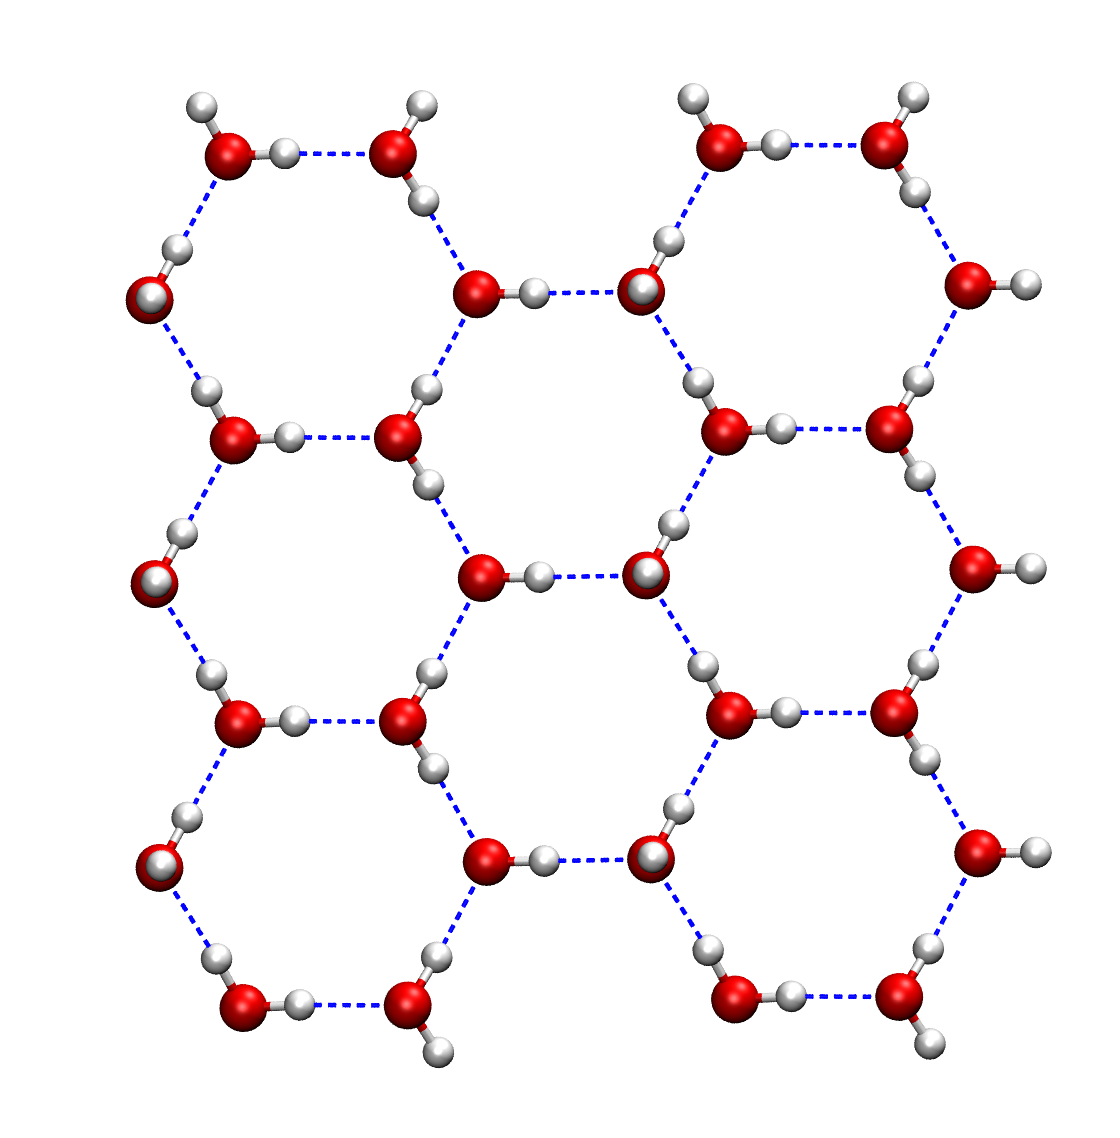
\includegraphics[width=.48\textwidth]{./img/FletcherAboveGlossyNoCueing.png}
\caption{The Fletcher surface. Hexagonal O (red) structure with vertical lines 
of identical H (white) orientation. H-bonds are indicated by dashed blue lines.
The O atoms are not all in the same plane.}
\label{Fig:Ads:Fletcher}
\end{figure}

It is given in Figure \ref{Fig:Ads:Fletcher}. Starting from a layer of
hexagonally arranged O atoms (which are not arranged on a plane but 
alteratingly above and below the plane), one can connect each O atom to its
four nearest neighbors. On these designated hydrogen bonds, H atoms can be placed close
to one of the two O atoms taking part in the bond. This can lead to a multitude
of possible arrangements. Fletcher's approach is to draw parallel
lines into the lattice to group the molecules in rows. Molecules in the
same row have the same orientation. In Figure \ref{Fig:Ads:Fletcher}, these
rows can be defined by vertical lines.

This ordering comes from first considering only the surface molecules. These
have a broken hydrogen bond outward, which may or may not have a hydrogen
atom on it. When grouping those broken bonds with hydrogen atoms and those
without hydrogen atoms in alternating rows, the structure described above is
extended to the full system.

Such a crystalline surface must be considered as an idealisation. For once,
since we are interested in an ice surface on a grain, the interaction between
the water molecules and the grain at the grain surface will surely lead to
changes in the surface, probably both in O position as well as in H orientation.
Research in that respect was presented by Cabrera Sanfelix
\etal\cite{CabreraSanfelix2003} on a graphite surface, where a water dimer
adsorbed on the surface has different bond angles than the gaseous water dimer.
Therefore, an undisturbed crystalline surface will only be reasonable if the
water ice is several monolayers thick, which is only the case in the cold
interstellar medium. A second idealization is that the crystalline structure of
water ice can only be true to the perfect hexagonal structure if a layer like in
Figure \ref{Fig:Ads:Fletcher} is wihtin the crystal, i. e. there are more such
layers above and below. Then, there is a balance of force. If the layers
above are removed to describe a surface layer, the forces from inside the crystal will
surely deform an ideal surface layer. We will see this effect in Section
\ref{Sec:Ads:Optima}.

\subsubsection{The QM/MM Region}
\label{Sec:Ads:QM/MM}
%% CHECK: Pics?
%% CHECK: what is prismatic surface? Thing in Fletcher?
%\tikzsetexternalprefix{TikzPics/Adsorption/}
%\tikzsetnextfilename{Fig.Ads.QMMM}

\begin{figure*}[ht]
\centering
%\newline
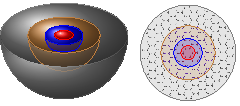
\includegraphics[width=\textwidth]{TikzPics/TikzCreation/SurfaceQMMM/SurfaceQMMMAside.pdf}
\newline
%\caption{The QM/MM division of the Fletcher surface. The upper picture shows the surface from above,
%the picture below is a schematic representation. The gray and the brown area make up the MM region,
%where water molecules are described by the $\tip$ potential. In the gray region, they are frozen. 
%The blue and brown region make up the QM region. Atoms in the blue region are described by the
%$\tzvp$ basis set. The central ring in the red region uses the $\tzvpd$ basis set.}
\caption{The QM/MM decomposition of the Fletcher surface. The picture to the right shows the surface from above,
the picture to the left is a schematic representation. The gray and the brown area make up the MM region,
where water molecules are described by the $\tip$ potential. In the gray region, they are frozen. 
The blue and brown region make up the QM region. Atoms in the blue region are described by the
$\tzvp$ basis set. The central ring constituting the red region uses the $\tzvpd$ basis set.}
\label{Fig:Ads:QMMM}
\end{figure*}

Of a fully-ordered water $I_h$ crystal with a Fletcher surface, we take
a semispherical cut of radius $25~\Ang$ centered on the center of a hexagonal
ring of water molecules. We choose a normal basal surface as in
Figure \ref{Fig:Ads:Fletcher}, not a prismatic surface. The semispherical
cut does not separate $\hto$ molecules internally, instead an $\hto$ molecule
is fully incorporated in the system if its O atom is within the cutoff
radius. The full number of QM/MM water molecules in the system is
1151, with 1151 O atoms and 2302 H atoms.

The decomposition into QM/MM domains is described in Figure \ref{Fig:Ads:QMMM}.
At a sphere of radius $8~\Ang$ we separate the system into two domains. The
domain within this sphere is the QM domain and the domain outside of it
is the MM domain. 
The QM region contains three layers of molecules. On the surface layer,
there is the central hexagonal ring of water molecules and the six
rings adjacent to it. The second layer has a water ring and the six
molecules forming hydrogen bonds with the O atoms of the ring. On 
the third layer, there is only one ring left. This would total
to 24+12+6=42 QM molecules. However, the QM description is only
necessary for regions where chemistry takes place. In our study,
this will all happen close to the surface. Therefore, going three
layers deep with the QM domain is not necessary and the the six
atoms of the lowest ring are also treated by MM. This makes the system slightly
less symmetric, but for the problems discussed here, the decrease in
computation time is enough to make up for that: calculations with 42 QM molecules
take on average 1.4 times as long as calculations with 36 QMmolecules.
Therefore, we decide on a total of 36 QM molecules. 
Of these, only the central ring at
the surface is described by the $\tzvpd$ basis set, the rest
uses the $\tzvp$ basis set. 

As for the MM domain, it is again separated at $15~\Ang$ of the system center.
Those molecules within that radius can change their position (active molecules) in the optimisations we
later carry out. The rest of the MM molecules is fixed in position (frozen molecules) to yield
%% CHECK: envelope? shell?
boundary conditions. The $10~\Ang$ envelope of frozen molecules may not be necessary as a boundary,
but on the other hand it has virtually no effect on computation time to include
these additional MM atoms, and if necessary they can be turned into
further active atoms. There is a total of 1121 MM molecules, of
which 231 are active MM molecules and 890 frozen MM molecules.

The geometry of the original Fletcher surface has to be changed to fit the requirements
of the $\tip$ potential. In the original formulation the hydrogen atoms
are placed directly on the hydrogen bonds, that is connecting lines between each oxygen atom
and its four nearest neighbors. This process yields bond angles of $109.50 \degree$
with a in princple variable bond length. The latter can be easily adjusted
to the $\tip$ requirements by simple stretching. This does not change the bond angles which
are still in disagreement with the bond angles of the $\tip$ potential
fixed at $104.52 \degree$. This is mended by simply taking a perfect
Fletcher surface with adjusted bond lenghts $\abs{\r_{\te O - \te H1}}=\abs{\r_{\te O - \te H2}}=0.9572~\Ang$
and changing the angles to the appropriate value while maintaining
the orientation of the water dipole moment, that is the vector $\r_{\te O - \te H1}+\r_{\te O - \te H2}$
stays the same for each molecule. This means symmetrical bending of all bond angles with
respect to the dipole moment.

\subsection{First Geometry Optimisations}
\label{Sec:Ads:Optima}

To verify the agreement between the theoretically assumed Fletcher surface and the
methods we want to use on it, we calculated RMSD values \eqref{Bench:RMSD} between
the ideal Fletcher surface and the surface it changes into after QM/MM optimisation.
Note that the factor $\frac 1 M$ in \eqref{Bench:RMSD} is not defined by the full number of QM/MM atoms
in the system but by the number of active QM/MM atoms.

% Table generated by Excel2LaTeX from sheet 'Tabelle1'
\begin{table}[t]
  \centering
  \caption{RMSD values for the all classical calculation with $\tip$ and
   QM/MM calculations with different functionals. The results are ordered
   with increasing RMSD.}
      \begin{tabular}{lr|lr}
    \tip  & \multicolumn{3}{l}{0.179 $\Ang$} \\[.2 pt]
    \hline
    \hline
    \bhlyp & 0.182 $\Ang$ & \pw\dt & 0.187 $\Ang$\\
    \btlyp & 0.183 $\Ang$ & \pbez & 0.193 $\Ang$\\
    \pw   & 0.183 $\Ang$ & \tpssh & 0.191 $\Ang$ \\[.2 pt]
    \hline
    \end{tabular}
  \label{Tab:Ads:RMSD.Methodcompare}%
\end{table}%

Data for the RMSD values are presented in Table \ref{Tab:Ads:RMSD.Methodcompare}. 
We include the pure MM optimisation with $\tip$. Generally,
the results can be considered good. For all systems, the same effect is visible: the
active $\hto$ molecules sink slightly into the surface. We did already have reasons
to expect that, as explained in Section \ref{Sec:Ads:Surface}.
%This can be expected, since
%the initial geometry is gained by cutting a perfect crystal at a plain, so the molecules
%that are now at the surface do not feel the attractive hydrogen bonds of the removed
%molecules anymore and move closer to the remaining molecules within the surface. 
This effect is not sinking process leads to an RMSD of order $< 0.2~\Ang$, and the displacement
is stronger the further a molecule is away from the frozen molecule region. Below
the surface layer, the displacements due to this effect are not very strong.

The RMSD among the DFT optima is very small, $0.035~\Ang$ and less. Even those
functionals we excluded in the benchmark yield optimum geometries within 
boundaries of an RMSD of $0.063~\Ang$. Between the functionals of Table \ref{Tab:Ads:RMSD.Methodcompare}
and the $\tip$ potential, there is an RMSD of roughly $0.1~\Ang$. The source of
this deviation is that the DFT water does not have the $\anghoh$ bond angle that
$\tip$ water has to satisfy.

We can therefore say that the QM/MM descriptions we decided on in this
and the previous section all find an optimum geometry that is close enough
to the ideal Fletcher geometry. 

%% Next part necesary?
\tikzsetexternalprefix{TikzPics/Adsorption/}
\tikzsetnextfilename{Fig.Ads.QMMMConvergence}
\begin{figure}[h]
\centering
 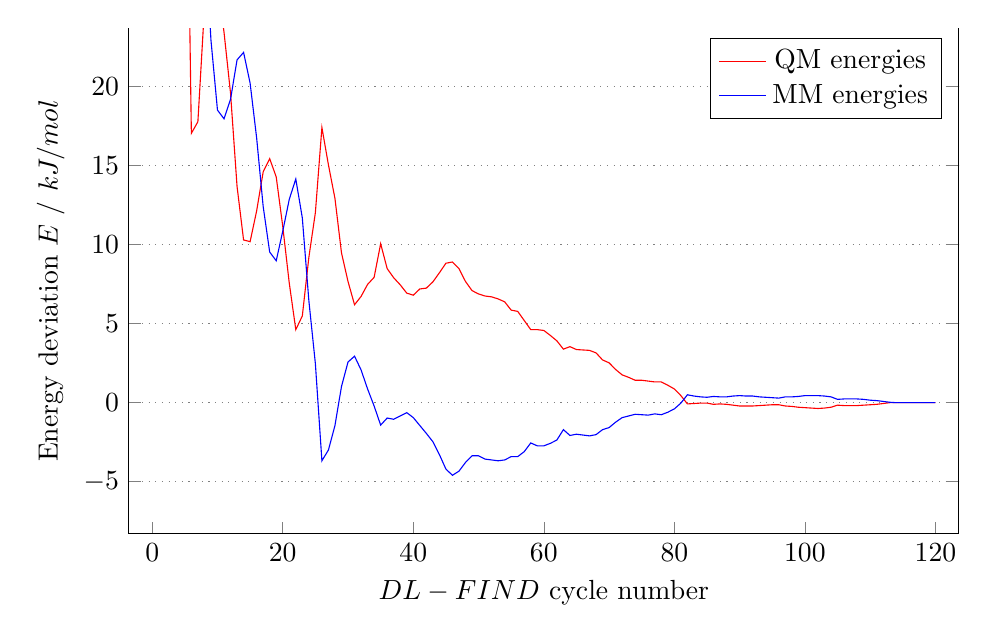
\begin{tikzpicture}
\begin{axis}[
    height=8cm,
    width=\linewidth,
    axis x line*=bottom,
    enlarge x limits=0.03,
    xmin=0,
    xmax=120,
    enlarge y limits=0.15,
    ymax=20,
    xtick={0,20,40,60,80,100,120},
    ylabel={Energy deviation $\Dl E$ / $\kmo$},
    xlabel={$\dlfind$ cycle number},
    grid style={dotted,gray},
    ymajorgrids=true,
    ]
\addplot[red] coordinates {(0,225.924275) (1,221.644710) (2,187.276915) (3,138.232575) (4,72.201250) (5,45.421150) (6,17.039495) (7,17.774635) (8,24.942250) (9,27.488985) (10,26.543805) (11,23.445715) (12,19.586230) (13,13.678855) (14,10.291960) (15,10.186940) (16,12.129810) (17,14.597780) (18,15.437940) (19,14.282720) (20,11.158375) (21,7.561440) (22,4.620880) (23,5.487295) (24,9.189250) (25,12.024790) (26,17.407065) (27,15.044115) (28,12.917460) (29,9.478055) (30,7.666460) (31,6.196180) (32,6.721280) (33,7.482675) (34,7.929010) (35,10.055665) (36,8.480365) (37,7.902755) (38,7.456420) (39,6.931320) (40,6.800045) (41,7.193870) (42,7.246380) (43,7.640205) (44,8.217815) (45,8.821680) (46,8.900445) (47,8.480365) (48,7.666460) (49,7.088850) (50,6.878810) (51,6.747535) (52,6.695025) (53,6.563750) (54,6.379965) (55,5.854865) (56,5.776100) (57,5.198490) (58,4.620880) (59,4.620880) (60,4.568370) (61,4.253310) (62,3.911995) (63,3.386895) (64,3.544425) (65,3.360640) (66,3.334385) (67,3.308130) (68,3.150600) (69,2.704265) (70,2.520480) (71,2.100400) (72,1.759085) (73,1.601555) (74,1.417770) (75,1.417770) (76,1.365260) (77,1.312750) (78,1.312750) (79,1.102710) (80,.866415) (81,.446335) (82,-.078765) (83,-.052510) (84,-.026255) (85,-.026255) (86,-.105020) (87,-.078765) (88,-.105020) (89,-.157530) (90,-.210040) (91,-.210040) (92,-.210040) (93,-.183785) (94,-.157530) (95,-.131275) (96,-.131275) (97,-.210040) (98,-.236295) (99,-.288805) (100,-.315060) (101,-.341315) (102,-.367570) (103,-.341315) (104,-.288805) (105,-.157530) (106,-.183785) (107,-.183785) (108,-.183785) (109,-.157530) (110,-.131275) (111,-.105020) (112,-.052510) (113,0) (114,0) (115,0) (116,0) (117,0) (118,0) (119,0) (120,0) };
\addplot[blue] coordinates {(0,42.979435) (1,42.506845) (2,37.518395) (3,31.427235) (4,39.408755) (5,48.598005) (6,58.548650) (7,46.471350) (8,30.403290) (9,22.946870) (10,18.509775) (11,17.958420) (12,19.192405) (13,21.686630) (14,22.159220) (15,20.216350) (16,16.750690) (17,12.418615) (18,9.530565) (19,8.979210) (20,10.843315) (21,12.864950) (22,14.151445) (23,11.683475) (24,6.458730) (25,2.467970) (26,-3.675700) (27,-2.993070) (28,-1.444025) (29,1.023945) (30,2.572990) (31,2.940560) (32,2.074145) (33,.866415) (34,-.210040) (35,-1.417770) (36,-.971435) (37,-1.050200) (38,-.840160) (39,-.630120) (40,-.945180) (41,-1.444025) (42,-1.942870) (43,-2.467970) (44,-3.281875) (45,-4.200800) (46,-4.594625) (47,-4.332075) (48,-3.780720) (49,-3.360640) (50,-3.360640) (51,-3.570680) (52,-3.623190) (53,-3.675700) (54,-3.623190) (55,-3.413150) (56,-3.413150) (57,-3.098090) (58,-2.546735) (59,-2.730520) (60,-2.730520) (61,-2.572990) (62,-2.362950) (63,-1.706575) (64,-2.074145) (65,-1.995380) (66,-2.047890) (67,-2.100400) (68,-2.021635) (69,-1.706575) (70,-1.575300) (71,-1.233985) (72,-.945180) (73,-.840160) (74,-.735140) (75,-.761395) (76,-.787650) (77,-.708885) (78,-.761395) (79,-.603865) (80,-.393825) (81,-.026255) (82,.498845) (83,.420080) (84,.367570) (85,.341315) (86,.393825) (87,.367570) (88,.367570) (89,.420080) (90,.446335) (91,.420080) (92,.420080) (93,.367570) (94,.341315) (95,.315060) (96,.288805) (97,.367570) (98,.367570) (99,.393825) (100,.446335) (101,.446335) (102,.446335) (103,.420080) (104,.367570) (105,.210040) (106,.236295) (107,.236295) (108,.236295) (109,.210040) (110,.157530) (111,.131275) (112,.078765) (113,.026255) (114,0) (115,0) (116,0) (117,0) (118,0) (119,0) (120,0) };
\legend{QM energies, MM energies}
\end{axis}
\end{tikzpicture}
\caption{The QM/MM energy changes during a typical optimisation. The 
energies are deviations from their value at the optimum geometry.
Functional: $\bhlyp$.}
\label{Fig:Ads:QMMMConvergence}
\end{figure}

We can also compare the behaviour of the QM and MM part during the optimisation
process starting at the initial crystalline geometry. Figure \ref{Fig:Ads:QMMMConvergence}
gives a typical example with the $\bhlyp$ functional. Both QM and MM energies are differences to
their values at the energy minimum. At the fully crystalline system, the
energy difference is too high for the plot axis, it goes up to $226~\kmo$ for the
QM part and $43~\kmo$ for the MM part. This is again an implication that the actual
optimum geometry has to be tighter bound and that the effect is strongest for the
QM region, although the high energies in the QM region must also be due to the
wrong geometry. After the first few iterations, one can see that the
energy changes in both domains are of the same order of magnitude. There is a codependence visible
where a more attractive interaction in the MM region is accompanied by a
less attractive interaction in the QM region and vice versa. We take
this as an implication that the interaction between the two region works
well and that neither one of them is outbalanced by too strong energy
gradients in the other one. We also see this as an indication that active MM atoms
should be included in a geometry optimization.

\subsection{ZPE Corrections}
\label{Sec:Ads:ZPE}

Now we have established a model that should be able to describe at least $\tripo$, 
H and $\hto$ adsorption to some satisfaction. We can compute optimum geometries
and their energies for different adsorbates and gain the adsorption energy
according to \eqref{Theo:AdsorptionEnergy}. Before we do so, it is necessary
to give a few words on the ZPE correction in this case.

Due to the QM/MM coupling, no analytical Hessian matrices can be computed.
There is no way around computing finite differences, so two atomic
diplacements per coordinate per atom, leading to six displacements
for each atom. Computations for more complicated systems, especially $\sur\hot$ calculations
with their dublet character, require a sensible choice
of atoms to be displaced. On the other hand of course, enough atoms should
be displaced such that the finite difference maintains good results.

Obviously, the MM atoms do not need to be displaced. If their electrons are not
described by quantum mechanics then neither should their atomic cores get a
quantum mechanical correction. As for the QM region, we come back to the argument that
the atoms relevant to adsorption are the central ring of six $\hto$ molecules plus adsorbate,
that is those atoms that we do describe with the $\tzvpd$ basis set. The idea
here is that when an adsorbate comes into the system and is adsorbed within the
central ring, then its impact on the vibrational ground state of the system
will mostly affect the atoms within the ring. The effect on atoms further
away should be considerably less. However, the question if the cutoff for this effect
should only include the central ring must be further investigated. The
upshot is obvious: With $M$ being the number of atoms in the adsorbate, these $18+M$ atoms
need $54+3M$ displacements (plus one initial geometry). This is much less than the
original $324+3M$ displacements for $108+M$ QM atoms.

We will call this selective correction the $\zpering$ correction in contrast to
the $\zpeall$ correction for all QM atoms. Corresponding energies are then called
$\ering$ and $\eall$, respectively, and the corrections are $\Dl\eall$ and $\Dl\ering$. 

We can compare the two corrections in the next section.


%% CHECK: Formation energies gegeneinander plotten? Eigentlich nicht sinnvoll,
%   da die QM Geometrien ja nicht unabhängig von den MM Geometrien sind.

\subsection{Adsorption}
\label{Sec:Ads:Adsorption}
\newcommand\avg{\enmat{E_{\te {avg}}}}
%If we assume the $\zpeall$ correction 
%to be accurate, we can evaluate the $\zpering$ correction when comparing
%results for the $\btlyp$ functional in Table \ref{Tab:Ads:AdsB3lyp}.
Of the molecules relevant in Section \ref{Sec:Gas}, we examine adsorption
%% CHECK: Conformation wirklich richtig? Chemisorption richtig? Unterschiede
%   zu Physisorption behandeln?
energies for all species but $\singo$, since it is chemisorbed by the surface
to form some conformation of $\htot$. This is a result of the barrierless
and very exothermic reaction $\hto+\singo\chemar\htot$, as described in
\eqref{Gas:H2O+O->H2O2}.

%% CHECK: Vllt lieber die Corrections als die Energiewerte?
\renewcommand\eads[1]{E_{\sur\te X}^{\te{ads}{#1}}}
\begin{table}[htb]
  \caption{Different choices for the ZPE correction. For a reference, the corresponding 
  adsorption energies are given for the $\btlyp$ functional. All energies in $\kmo$.}
  \centering
    \begin{tabular}{l|rrrr}
       & & & & \\[-10pt]
     & $E_{\btlyp}$   & $\Dl\eall_{\btlyp}$ & $\Dl\ering_{\btlyp}$ & $\Dl\ering_{\pbez}$ \\[2pt]
    \hline
       & & & & \\[-10pt]
    $\sur\te{H}$ & $-$1.71 & 5.03  & 3.28  & 2.84 \\
    $\sur\htw$ & $-$2.65 & 8.42  & 6.80  & 6.81 \\
    $\sur\hto$ & $-$48.01 & 15.98 & 14.84 & 14.45 \\
    $\sur\htot$ & $-$41.76 & 9.28  & 10.09 & 9.51 \\
    $\sur\ho$ & $-$44.99 & 13.60 & 12.11 & 12.05 \\
    $\sur\hot$ & $-$65.48 & 13.17 & 11.66 & 11.59 \\
    $\sur\tripo$ & $-$16.17 & 2.69  & 3.35  & 3.04 \\
    $\sur\singot$ & $-$8.41 & 2.46  & 3.86  & 4.96 \\
    $\sur\tripot$ & $-$2.62 & 3.06  & 3.90  & 3.86 \\[2pt]
    \hline
    \end{tabular}%
% \begin{tabular}{l | r|r|r|}
% & & & \\[-10pt]
%     & \ph{$^{\zpeall}$}$\eads{}$ & $\eads{,\zpering}$ & $\eads{,\zpeall}$ \\[2pt]
%     \hline
%        & & & \\[-10pt]
%     $\sur\te H$ & -1.69 & 1.62  & 3.43 \\
%     $\sur\te H_2$ & -2.65 & 4.19  & 5.91 \\
%     $\sur\hto$ & -48.00 & -33.14 & -32.06 \\
%     $\sur\htot$ & -41.76 & -31.62 & -32.39 \\
%     $\sur\te{HO}$ & -44.98 & -32.85 & -31.39 \\
%     $\sur\te{HO}_2$ & -65.48 & -53.79 & *** \\
%     $\sur^3\te O$ & -16.15 & -12.77 & -13.38 \\
%     $\sur^1\te O_2$ & -8.42 & -4.50 & -5.76 \\
%     $\sur^3\te O_2$ & -2.48 & 1.49  & 0.83 \\[2pt]
%     \hline
%     \end{tabular}
  \label{Tab:Ads:AdsB3lyp}%
\end{table}%

%% CHECK: Wird das noch was?
%Also note that the $\hot$ calculation did not finish within the six days
%of computation on the JUSTUS cluster for the $\zpeall$ correction. It did
%only finish 307 of 333 displacements.  

Before discussing adsorption data, we want to discuss the relevance of the
$\zpe$ correction and the differences between $\zpeall$ and $\zpering$
as well as the differences between the $\zpering$ correction for $\btlyp$ and
$\pbez$, which we hope to represent the general variability of the
$\zpe$ correction for different functionals.

In general, the value of the corrective term does vary from
adsorbate to adsorbate. All three corrections lie roughly between $2$
and $16~\kmo$. That makes them -- if there is no cancellation
of error of some other sort -- necessary for the correct description
of adsorption processes, since the uncorrected adsorption energies
themselves lie between $-1.71$ and $-65.48~\kmo$. The value of the 
ZPE correction is also typically greater than the variation of
the uncorrected adsorption energy of different functionals, as we
can see when comparing to Table \ref{Tab:Ads:AdsForFuncs}.

The $\zpeall$ and $\zpering$ energies
do not deviate strongly in absolute value, all of them less than $2~\kmo$
and all but $\sur$H and $\sur$HO by less than $1.5~\kmo$. All corrections are
positive.
% and in most cases the deviation is of less than 25\% between
%the two. Only for $\sur$H and $\sur^1\ot$ the deviations are greater than 35\%.
It seems safe to say that the $\zpering$ correction may not be extremely
close to the $\zpeall$ correction, but it shows the same qualitative
behaviour. And since there is no knowing whether or not $\zpeall$ is
accurate either, it seems alright to use the correction of the smaller
system while accepting error bars of $\pm 2~\kmo$.

Comparing the corrective terms for $\btlyp$ and $\pbez$, we generally find
good agreement. With the exception of $\sur^1\ot$, the energies
differ by less than $0.6~\kmo$.
%The case of $\sur^1\ot$ is also
%interesting because it is the only case where the $\pbez$ correction
%predicts a greater value than the $\btlyp$ correction.
Given the uncertainty between $\zpering$ and $\zpeall$, the differences
between the  $\pbez$ correction and the $\btlyp$ correction are negligible.
It seems reasonable to generalize what we already discovered for the gas
phase result of Section \ref{Sec:Gas}: the ZPE correction does
not change greatly between different functionals. We will therefore
use the $\zpeall$ correction for the $\btlyp$ functional for all
following data.

Talking about the differences between $\zpe$ corrected adsorption energies
and those without correction, there are the interesting cases of 
$\sur$H, $\sur\htw$ and $\sur\tripot$. In all three cases, the uncorrected
$E$ predicts attractive interaction, while the corrected $\eall$
and $\ering$ both predict repulsive interaction. That means that
the binding site found by the uncorrected DFT method is probably not the
desired optimum.
In such a case, it would of
course be interesting whether there is an optimum geometry for the $\zpe$
corrected functional that is still attractive. One should assume so,
since it would seem unphysical if the surface and one of the
molecules would repel one another. The problem here may be more the
$\btlyp$ functional than the $\zpe$ correction alone. Due to the computational
cost of a single ZPE correction, an optimization on a more sophisticated 
PES will be very difficult to achieve.

In any case, it is safe to say that the adsorbates $\sur$H, $\sur\htw$ and $\sur\tripot$
are only very weakly bound to the surface.

% We can further evaluate the significance of the ZPE correction by comparing
% it to the variation in (uncorrected) adsorption energy among 
% the different functionals.

\newcommand\tableskip{\hskip 0pt}
\newcommand\leftattable{\raggedright\hskip 53pt}
\newcommand\righttable{\raggedleft}
\newcommand\righttablestop{\hskip-53pt}
\newcommand\footnotebox{\tableskip\tableskip\makebox[.93\textwidth][r]}
%% CHECK: b3lyp muss ja evtl nicht nochmal a	usgegraben werden. Dafür
% vllt pw6b95.
%% CHECK: More Experiments?
%% CHECK: Deviation from average value? 
% Table generated by Excel2LaTeX from sheet 'Tabelle1'
\begin{table*}[ht]
  \centering
  \caption{Comparison of adsorption energies for different density functionals. All
  energies are given with $\zpeall$ correction for $\btlyp$. $\pws$ is shorthand
  for $\pw$. Energies can be compared to the average $\avg$ (excluding $\pws\dt$)
  and experimental data. Energies in $\kmo$.}
    %\begin{tabular}{l|L{2cm}L{2cm}L{2cm}L{2cm}L{2cm}}
    \begin{tabular}{l|rrrrrr|r|r}
    & & & & & & & & \\[-10pt]
          & \btlyp & \bhlyp & \pbez & \tpssh & \pws & \pws\dt & $\avg$ &experimental, $E_\te{des}$\\[2pt]
    \hline
       & & & & &  & & & \\[-10pt]
    $\sur\te{H}$ & 3.32  & 3.77  & 3.37  & -5.05 & 3.29  & 1.27 & 1.74 & \\
    $\sur\htw$ & 5.77  & 5.11  & 3.57  & 4.55  & 4.65  & 2.47 & 4.73 & \\
    $\sur\hto$ & $-$32.03 & $-$35.07 & $-$36.90 & $-$30.92 & $-$33.51 & $-$41.17 & $-33.69$ & $-$$48.00\pm0.50$\fakefna\\
    $\sur\htot$ & $-$32.47 & $-$35.99 & $-$37.64 & $-$31.04 & $-$34.85 & $-$44.33 & $-34.40$ &\\
    $\sur\ho$ & $-$31.39 & $-$32.88 & $-$35.69 & $-$31.10 & $-$32.78 & $-$39.66 & $-32.77$ & $-$$13.77$ to $-$$39.58$\fakefnb\\
    $\sur\hot$ & $-$52.30 & $-$49.10 & $-$56.97 & $-$54.10 & $-$51.08 & $-$57.80 & $-52.71$ & \\%  $13.80\pm0.50$\fakefnb,\\
    %% CHECK: This value is only for the bare silicate
    %& & & & & & & $15.38\pm0.75$\fakefnb \\
    $\sur\tripo$ & $-$13.48 & $-$5.16 & $-$11.25 & $-$13.22 & $-$12.85 & $-$18.13 & $-11.19$ &
    $-13.80\pm0.50$, $-15.38\pm 0.75$\fakefnc \\
    $\sur\singot$ & $-$5.95 & $-$7.51 & $-$11.44 & $-$9.44 & $-$7.44 & $-$12.53 & $-8.36$ & \\
    $\sur\tripot$ & 0.45  & $-$0.65 & $-$1.52 & $-$0.52 & 26.68 & 7.04 & $-0.56^\dagger$ & $-$7.52\fakefnd\\[2pt]
    \hline
    \end{tabular}
    \\[5pt]
    \footnotebox{
    \fakefna\footnotesize Adsorption on Au grain covered in crystalline water. For other grain materials between $42.15$ and $49.79~\kmo$. Fraser $\etal~$ 2001\cite{Fraser2001}}\\
    %% CHECK: Überhaupt relevant, wenn nicht auf asw oder crystalline?
    \footnotebox{
    \fakefnb\footnotesize Adsorption on an amorphous silicate. He, Vidali 2014 \cite{HeVidali2014}}\\
    %% CHECK: Paper anschauen, LESEN
    \footnotebox{
    \fakefnc\footnotesize Adsorption on porous amorphous water ice and amorphous silicate, respectively. He $\etal~$ 2015 \cite{He2015}}\\
    \footnotebox{
    \fakefnd\footnotesize Adsorption on an amorphous silicate. He, Jing, Vidali 2014 \cite{HeJingVidali2014}}\\
    \footnotebox{
    $^\dagger$\footnotesize Average excluding both $\pws$ and $\pws\dt$.}\\
    %\makebox[10cm]{\ragggedleft Text}\\
    %\leftattable Text\\
    %\righttable\righttablestop Text
    %\raggedleft\fakefna\footnotesize Value for an Au grain. Value for other substrates between $42.15$ and $49.79~\kmo$.
  \label{Tab:Ads:AdsForFuncs}%
\end{table*}%

Let us now turn to Table \ref{Tab:Ads:AdsForFuncs}, where ZPE corrected adsorption
energies are given. Where there is experimental data available, it is given
in the last column. So far, not many studies exist on measuring 
adsorption under interstellar conditions. We therefore also included some data
for $\ho$, $\tripo$ and $\singot$ adsorption on bare amorphous silicates, which were gathered in order to
gain a better understanding of water ice formation on bare silicates \cite{HeVidali2014,HeJingVidali2014}.
Other data include $\hto$ adsorption on an Au surface covered in crystalline water
%% CHECK: Es müsste \tripot sein, da Bildungsenergie für \singot größer ist als für \tripot
%    Nein, ich glaube nicht, da die Adsorptionsenergie stärker ist für \singot, das heißt ein
%    adsorbiertes O wird eine \singot-Struktur suchen. Wahrscheinlich passiert das, bevor es desorbiert.
ice\cite{Fraser2001} and $\tripot$ adsorption on porous amorphous water ice \cite{He2015}.
%% CHECK: Wie sinnvoll ist das?
%Although the experiments on bare silicates do not quite resemble our system,
%we consider the data they provide to give good guidance since they are at least
%influenced by adsorption on the freshly formed water ice surfaces on the probes.
We have an estimation of the difference between adsorption on water ice and
on the bare grain by comparing the experimental data for $\sur\tripo$, where the difference
is below $3~\kmo$ including the error bars. While this does not have to apply to all
adsorbates, a difference of similar magnitude is at least plausible, such that
the experimental values for adsorption energies on bare grains should be a rough estimate
to the adsorption energies on water surfaces on grains.

% Also note that the experiments were measurements of the desorption energy. They are
% typically temperature-dependent. We did not include any dynamical effects into our
% computations, which means they are basically data at $0~\K$. At such low temperatures,
% the difference should  

% If we compare this data directly to the $\zpe$ corrections, we should bear in mind that the
% $\zpe$ corrections given so far are only values for the $\btlyp$ functional. It
% is however well possible that the corresponding corrections of other functionals
% are of similar magnitude, given that for many adsorbates, the adsorption energy
% does not vary too strongly between the functionals. Still, the difference
% between most attractive and most repulsive functional is often greater than
% either $\zpe$ correction. As long as there is no evidence that one
% of the functionals is more accurate than the others, the error
% from the uncertain choice of functional is of the same dimension as the error
% introduced by neglect of the $\zpe$ correction. Nonetheless, the $\zpe$
% correction should be included in calculations since it seems to introduce
% additional repulsion into the system. Especially if it does really expose
% bad choices of optimum geometry, i.e. binding sites, as for the case
% of $\sur^3\ot$ for $\btlyp$.

Table \ref{Tab:Ads:AdsForFuncs} also contains a column with average values
for each adsorbate. Due to its usual deviation from the other functionals,
$\pw\dt$ is not included into the averaging. For $\sur\tripot$, 
$\pw$ is aditionally excluded because of the very unphysical value of
$26.68~\kmo$. We will use this average energy when discussing reactions.

%% CHECK: Sehr schwammig hier.
Where there is no experimental data available, we can only compare the
functionals to one another. For both $\sur\te H$ and $\sur\htw$, the
problem of repulsive interaction due to ZPE correction seems to affect
most functionals. $\tpssh$ disagrees with the others by still maintaining
a negative sign for $\sur$H, but for $\sur\htw$, all functionals agree.
This is at least an indication that the physisorption of H and $\htw$ are
very fragile and that rather oxygen and hydrogenated oxygen species
have longer residence times than hydrogen.
For $\tripot$, the case is a little puzzling. $\pw$ predicts a strong
repulsion between surface and $\tripot$, which is supported by
$\pw\dt$. This looks like an error in input values, however we were
unable to find such an error. We must therefore consider $\pw$
to be to be unreliable for $\tripot$ adsorption. The other
functionals predict very weak attraction, only $\btlyp$ predicts
a very weak repulsion. We thus infer that $\tripot$, too, is
probably only weakly bound to the surface and must have a short
residence time.
% $^3\ot$, which was also
% critical in our discussion of the ZPE correction, is not the unanimously
% considered repulsive. The $\pw$ method predicts strong repulsion,
% which is to some extent supported by $\pw\dt$, but the rest of the functionals
% seems to still predict a weak attraction or in the $\btlyp$ case a very
% weak repulsion.

While each functional does have its ``slips'' for some adsorbates, the first four functionals of
Table \ref{Tab:Ads:AdsForFuncs} seem to be in good accord. 
For many cases, one of the two $\pw$ functionals is furthest from an average
value of all six functionals. This is especially true for O and $\ot$.
Since it is either $\pw$ or $\pw\dt$, this could be an indication
that neither the $\pw$ nor the D3 dispersion correction are universally
reliable for the study at hand. Of course, some of these possibly erroneous
results could stem from $\dlfind$ getting stuck in the wrong minima. 

Comparing the results to experimental findings, the agreement is more qualitative
than quantitative. As already mentioned, the systems described by experiment
differ from the idealized system we study. Most noteworthy is that the data for $\sur\hto$
is far off while the experiment yielding the results should be the one closest
to our model. The agreement would be better if we neglected $\Dl\eall=15.98$,
with extremely good results for $\btlyp$ (cf. Table \ref{Tab:Ads:AdsB3lyp}).
It is even the case that the experimental values mostly lie somewhere between
the $\zpe$ corrected energy value and the uncorrected one for many functionals.
But this should not question the reliability of the ZPE correction, since it
represents a physical necessity and is here carried out close to the best precision
available.
%% CHECK: Das nötig?
We should rather question sources of error like the system's strongly
idealized geometry, which is not only due to the QM description but also to
the water geometry of the MM description, which would make it difficult to
allow for systems with distorted bond angles as described by Cabrera Sanfelix $\etal~$ 
\cite{CabreraSanfelix2003} for the case of adsorption of a water dimer on graphite.
We will come back to possible improvements to the model in the final section.

% Compared to the experimental data, the case of $\tripot$ seems to be difficult
% to describe for all functionals. They predict weak adsorption, while the data by
% He \cite{He2015}, which is for an amorphous surface, predicts adsorption
% energies around $-13.8~\kmo$. While this could be dependent on the surface
% geometry, particularly bad  

On the other hand, the broad agreement between $\btlyp$, $\bhlyp$, $\pbez$
and $\tpssh$ allows for the assumption that the energies calculated for the
model at hand may be accurate to within a few $\kmo$. Since we chose
the functionals because they were best able to describe interaction
energies in Section \ref{Sec:Bench}, this hope becomes more plausible.
However, due to their rather bad performance for O species, the $\pw$
functionals have lost some credibility.


% Again, there is no knowing 
% what results are accurate. But if a single functional does not agree well with
% the rest of them, as is the case for $\pw\dt$, one could argue that it may
% at least be a little more off than the others. Also, the result
% of repulsive $\sur^3\ot$ interaction is odd, especially since $\pw\dt$ 
% expected too attractive interaction for the $\htoo$ benchmark.

% Concerning the other four functionals, one cannot make out many patterns
% in their behavior. They agree within $\pm2.5~\kmo$ of an average value
% for half of the adsorbates, but they do not coincide well for $\sur$H, $\sur\hot$,
% $\sur^3$O and $\sur^1\ot$, either because of a single functional strongly
% disagreeing or because of all functionals predicting energies in a broader
% area. There is no thoroughly satisfactory conclusion to this. One can
% at least argue qualitatively that the results should be physically
% sensible and that the scatter of possible values could be used as an error
% bound for the actual data.

\subsection{Reactions}
\label{Sec:Ads:Reactions}

%% CHECK: Durchschnittswert in nem Bild präsentieren? Durchschnittswert wirklich clever?
\newcommand\btlyps{\enmat{\te{B3}}}
\newcommand\pbezs{\enmat{\te{PBE0}}}
% Table generated by Excel2LaTeX from sheet 'Tabelle1'
\begin{table*}[htb]
  \centering
  \caption{Surface reaction energies with Eley-Rideal type reactions. All energies are $\zpe$ corrected with $\Dl E^{\zpeall}_\btlyp$.
  $\pws$ is short for $\pw$. The functionals most accurate for the gas phase
  reactions are highlighted by boldface again (cf. Table
  \ref{Tab:Gas:Reactions}). The last column contains average values.
  The deviations of these are listed in the last four rows for each functional.}
    \begin{tabular}{lll|rrrrrr|r}
        & & & & & & & &\\[-10pt]
        & &    & \btlyp & \bhlyp & \pbez & \tpssh & \pws
    & \pws\dt &  \multicolumn{1}{r}{$\avg$}  \\[2pt]
    %& &    & \btlyp & \bhlyp & \pbez & \tpssh & \pws   & \pws\dt &  $\Dl \eall_{\btlyps}$ & $\ering_{\btlyps}$ & $\Dl \ering_{\pbez}$ \\[2pt]
    \hline 
    & & & & & & & &\\[-10pt]
        $\sur\ho$&\defskip$+\te{H}\gas$&\defskip$\chemar\sur\hto$ & $-$476.22 &
        $-$458.03 & $-$472.39 & $-$470.76 & $\bo{-480.13}$ & $\bo{-480.92}$ &
        $-$473.07
        \\
    $\sur\hto$&\defskip$+^1\te{O}\gas$&\defskip$\chemar\sur\htot$ & $-$402.54 &
    $\bo{-357.85}$ & $-$427.27 & $-$426.38 & $-$405.24 & $-$407.50 & $-$404.46
    \\
    $\sur\ho$&\defskip$+\ho\gas$&\defskip$\chemar\sur\htot$ & $-$185.12 &
    $-$137.04 & $-$194.02 & $-$187.84 & $\bo{-197.12}$ & $\bo{-200.16}$ &
    $-$183.55
    \\
    $\sur\hot$&\defskip$+\te{H}\gas$&\defskip$\chemar\sur\htot$ & $\bo{-317.22}$
    & $-$318.69 & $-$310.31 & $-$309.82 & $-$320.89 & $-$323.99 & $-$316.82 \\
    $\sur\ho$&\defskip$+^3\te{O}\gas$&\defskip$\chemar\sur\hot$ & $-$294.05 &
    $-$219.54 & $-$300.54 & $\bo{-295.71}$ & $-$296.15 & $-$296.10 & $-$283.68
    \\
    $\sur^3\te{O}$&\defskip$+\ho\gas$&\defskip$\chemar\sur\hot$ & $-$311.96 &
    $-$248.31 & $-$325.41 & $\bo{-313.50}$ & $-$316.45 & $-$318.00 & $-$305.61
    \\
%    $\sur^1\ot$&\defskip$+\te{H}\gas$&\defskip$\chemar\sur\hot$ & $-$403.80 &
    % $-$414.31 & $-$402.88 & $-$404.70 & $-$395.22 & $-$396.95 & $-$402.98 \\
    $\sur^3\ot$&\defskip$+\te{H}\gas$&\defskip$\chemar\sur\hot$ & $-$248.05 &
    $-$243.27 & $-$241.72 & $\bo{-250.31}$ & $-$268.95 & $-$256.14 & $-$251.41
    \\[2pt]
    
    \hline \hline
\multicolumn{2}{r|}{\multirow{4}{*}{$E_{\dft} - \avg$}} &
       MAD   &     3.87  & 34.23 & 12.40 & 8.08  & 9.48  & 9.17  & \\
 \multicolumn{2}{r|}{} & MIN   & $-$10.37 & $-$1.87 & $-$22.81 & $-$21.91 & $-$17.54 & $-$16.61  & \\
 \multicolumn{2}{r|}{} & MAX   & 3.36  & 64.14 & 9.68  & 7.01  & $-$0.78 & $-$3.04 & \\
 \multicolumn{2}{r|}{} & MEAN  & $-$2.37 & 33.70 & $-$7.58 & $-$5.10 & $-$9.48 & $-$9.17  &  \\[2pt]
    %\\[-10pt]
    \end{tabular}%
    %\\
    %\raggedleft\fakefna\footnotesize Correction value for $\btlyp$ calculation. Others differ in $\ho\gas$ $\zpe$ correction within $1.5~\kmo$.
  \label{Tab:Ads:React}%
\end{table*}%


With the adsorption energy data and corresponding gas phase energies at the
$\tzvpd$ level, we can calculate reaction energies. We will only
consider reactions of the Eley-Rideal mechanism in which a molecule
from the surrounding gas approaches an adsorbed molecule to form
a new molecular species, as described in Section \ref{Sec:Theo:Interaction}.
The product will for our study always be a single adsorbed molecule. With our data,
one could also investigate cases where two product molecules remain
of which none, one or both remain adsorbed on the surface.

We use Eley-Rideal versions of the gas phase reaction \eqref{Gas:Reactions}, namely

\renewcommand\ronebox[1]{\makebox[1cm][l]{\enmat{#1}}}
\renewcommand\rtwobox[1]{\makebox[1.cm][l]{\ \enmat{#1}}}
\renewcommand\prodbox[1]{\makebox[1.65cm][l]{\enmat{#1}}}
\begin{subequations}
\begin{align}
   \label{Surf:HO+H->H2O}
   \ronebox{\sur\ho}+\rtwobox{\te{H}\gas}\prodbox{\chemar\sur\hto,} \\ 
   \label{Surf:H2O+O->H2O2}
   \ronebox{\sur\hto}+\rtwobox{\singo\gas}\prodbox{\chemar\sur\htot,} \\
   \label{Surf:HO+HO->H2O2}
   \ronebox{\sur\ho}+\rtwobox{\ho\gas}\prodbox{\chemar\sur\htot,} \\
   \label{Surf:HO2+H->H2O2}
   \ronebox{\sur\hot}+\rtwobox{\te{H}\gas}\prodbox{\chemar\sur\htot,} \\
   \label{Surf:HO+O->HO2}
   \ronebox{\sur\ho}+\rtwobox{\tripo\gas}\prodbox{\chemar\sur\hot,} \\
   \label{Surf:O+HO->HO2}
   \ronebox{\sur\tripo}+\rtwobox{\ho\gas}\prodbox{\chemar\sur\hot,} \\
%    \label{Surf:1O2+H->HO2}
%    \ronebox{^1\ot}+\rtwobox{\te{H}}\prodbox{\chemar\hot,} \\
   \label{Surf:3O2+H->HO2}
   \ronebox{\sur\tripot}+\rtwobox{\te{H}\gas}\prodbox{\chemar\sur\hot.}
\end{align}
\label{Surf:Reactions}
\end{subequations}

Note that both \eqref{Surf:HO+O->HO2} and \eqref{Surf:O+HO->HO2} are Eley-Rideal
versions of \eqref{Gas:HO+O->HO2}, but with different reactant adsorbates.

The reaction energies for \eqref{Surf:Reactions} are given in Table \ref{Tab:Ads:React}.
All reaction energies are computed according to \eqref{Theo:ReactionEnergySurface}.

For each molecule, we use the energy values at the optimized geometries of each functional plus
the $\zpeall$ correction with the $\btlyp$ functional. Note that we have an ambiguity in the choice
of $\zpe$ corrections for the reactions with $\ho\gas$. This is the only
case where the gaseous reactant does have a non-vanishing $\zpe$ correction.
This means that we can either use the corrective term demanded by the
individual functional or always the one demanded by $\btlyp$. We chose to use
%% CHECK: richtige Wahl?
the $\btlyp$ correction for the $\ho\gas$ molecules, too, which makes the whole
ZPE correction more consistent. This choice may be challenged, however it 
changes the energy of the two reactions at hand by never more than $1.05~\kmo$,
and this biggest change appears for $\bhlyp$, which is generally not in good
agreement with the rest of the reaction energies anyway.

Recalling the strong deviations between DFT and $\ccsdtf$ gas phase
reaction energies, we must admit that we can not know which of
the DFT reaction eneriges in table \ref{Tab:Ads:React} is close to the truth.
To still make some qualitative inferences, we chose two approaches. The
first one is that we highlight the most accurate functional in the
gas phase for each reaction, cf. Table \ref{Tab:Gas:Reactions}. Since we do not
know in which cases the D3 correction may be an improvement, we always
highlight both values for the $\pw$ functional. We already explained that
there is no evidence for functionals maintaining the accuracy of the gas
phase results, but at least a functional with strong deficiencies in
the gas phase is not particularly qualified to a surface reaction either, while
a more accurate functional in the gas phase has a chance of acceptable results
for adsorbed molecules. 

The second option for recommendations is an average adsorption energy for each reaction. There is
also no reason to hope that the process of averaging should help to find
an accurate value for the reaction energy, especially since the
$\dft$ gas phase reaction energies were often incongruent with the $\ccsdtf$ data.
%% CHECK: Langer Satz, unsinnig.
% The sample of reactions is also too small to claim that a functional
% that is close to the average in most cases should be close to the average
% value of DFT energies for all surface reactions composed of these molecular
% species.

But to offer recommendations for reaction energies which may be of further
use to simulations, it seems reasonable to provide a value that is somewhat
representative to the data of all functionals. And since there is no
clear implication which functional may yield energies closest to the actual
rection energy for each case, the choice of taking a simple mean value comes naturally.

We can calculate the MAD from the average values, which is minimal for the $\btlyp$ functional.
With a maximum absolute deviation of $10.37~\kmo$, $\btlyp$ can be seen as not too strongly
varying.

Note that neither the average nor the most accurate gas phase functional give recommendations
of which functional to use for similar reactions. If one follows the gas phase functional
approach, each new reaction has to be evaluated by a gas phase test before a functional
for the surface reaction can be chosen. As for the average, the small set of
reactions can not be representative of the large variety of surface reactions,
even if one only allowed for molecular species composed of H and O. 

After these preliminary comments on functional recommendations, we want to look at the
specific reactions. The difference between a surface reaction and a gas phase reaction
for the reactions we study is exactly the difference between the adsorption energy
of the adsorbed product and the adsorbed educt. Therefore, the similar adsorption
energies of $\sur\ho$, $\sur\hto$ and $\sur\htot$ cause similar reaction energies
for the first three reactions in the gas phase as well as on the surface. 

\section{Possible Application}
\subsection{Binding Sites}
\label{Sec:Adv:Binding}


\subsection{Transition State and IRC}
\label{Sec:Adv:IRC}
%% CHECK: Theory entry

\newpage

\section{Conclusion}
\label{Sec:Con}

\section*{Acknowledgment}
I want to thank Professor J. Kaestner for his support and Mr. Jan Meisner for
his introduction to the topic and his company along the way.


%\clearpage
% \bibliographystyle{apalikenotitle}
\bibliographystyle{ieeetr}
% \begin{thebibliography}
%\bibliography{MasterBib}
\bibliography{ShortTitles,MasterBib}{}
\end{document}